\chapter{پیشینه پژوهش}

\section{مقدمه}
ظهور مدل‌های Transformer و انقلاب در یادگیری عمیق، یکی از تحولات اساسی در حوزه پردازش زبان طبیعی (NLP) و یادگیری ماشین به شمار می‌رود. این مدل‌ها باعث تغییرات عمده‌ای در نحوه ساخت و آموزش مدل‌های زبانی و همچنین در بسیاری از کاربردهای دیگر یادگیری ماشین شده‌اند. و توانستند بسیاری از مشکلات مدل های قبلی را حل کنند.

\section{مشکلات ترجمه ماشینی و ترانسفورمرها:}
در ابتدا، ترجمه ماشینی (MT) یک چالش اساسی در زمینه پردازش زبان طبیعی بود. مدل‌های اولیه‌ای مانند مدل‌های مبتنی بر قواعد (Rule-based models) برای ترجمه استفاده می‌شدند که در آن‌ها، ترجمه‌ها به صورت دستی با استفاده از قواعد زبانی مشخص تنظیم می‌شدند.
این روش‌ها هرچند دقیق بودند، اما محدودیت‌های زیادی داشتند و نمی‌توانستند ویژگی‌های پیچیده‌تر زبان را مدل‌سازی کنند.
سپس مدل‌های آماری (Statistical Models) معرفی شدند. این مدل‌ها از داده‌های ترجمه‌شده برای آموزش مدل‌های آماری استفاده می‌کردند که احتمال ترجمه‌ای صحیح را براساس شواهد آماری محاسبه می‌کردند. مدل‌هایی مانند مدل‌های ترجمه آماری مبتنی بر جمله (Phrase-based Statistical Models) از این نوع بودند، که قادر به ترجمه جملات بهتر از مدل‌های مبتنی بر قواعد بودند، اما هنوز هم در ترجمه‌های پیچیده با مشکلاتی روبه‌رو بودند.  بعد از این مدل ها مدل ها بازگشتی به وحود آمدند که مشکلات آن را در فصل گذشته بیان کردیم و د نهایت این مشکلات باعث به وجود آمدن ترانسفورمر ها شد.\section{مقدمه}
ظهور مدل‌های Transformer و انقلاب در یادگیری عمیق، یکی از تحولات اساسی در حوزه پردازش زبان طبیعی (NLP) و یادگیری ماشین به شمار می‌رود. این مدل‌ها باعث تغییرات عمده‌ای در نحوهٔ ساخت و آموزش مدل‌های زبانی و همچنین در بسیاری از کاربردهای دیگر یادگیری ماشین شده‌اند و توانستند بسیاری از مشکلات مدل‌های قبلی را حل کنند.

\section{مشکلات ترجمه ماشینی و ترانسفورمرها}
در ابتدا، ترجمه ماشینی (MT) یک چالش اساسی در زمینهٔ پردازش زبان طبیعی بود. مدل‌های اولیه‌ای مانند مدل‌های مبتنی بر قواعد (\lr{Rule-based Models}) برای ترجمه استفاده می‌شدند که در آن‌ها، ترجمه‌ها به‌صورت دستی با استفاده از قواعد زبانی مشخص تنظیم می‌شدند. این روش‌ها هرچند دقیق بودند، اما محدودیت‌های زیادی داشتند و نمی‌توانستند ویژگی‌های پیچیده‌تر زبان را مدل‌سازی کنند.

سپس مدل‌های آماری (\lr{Statistical Models}) معرفی شدند. این مدل‌ها از داده‌های ترجمه‌شده برای آموزش مدل‌های آماری استفاده می‌کردند که احتمال ترجمهٔ صحیح را براساس شواهد آماری محاسبه می‌کردند. مدل‌هایی مانند مدل‌های ترجمهٔ آماری مبتنی بر جمله (\lr{Phrase-based Statistical Models}) از این نوع بودند که قادر به ترجمهٔ جملات بهتر از مدل‌های مبتنی بر قواعد بودند، اما هنوز هم در ترجمه‌های پیچیده با مشکلاتی روبه‌رو بودند.

بعد از این مدل‌ها، مدل‌های بازگشتی (\lr{Recurrent Models}) به وجود آمدند که مشکلات آن‌ها در فصل گذشته بیان شد. در نهایت، این مشکلات باعث به وجود آمدن ترانسفورمرها شد.

\section{ظهور ترانسفورمرها}
در سال ۲۰۱۷، مقاله‌ای توسط گوگل منتشر شد که مفهوم جدیدی به نام ترانسفورمرها را معرفی کرد. این مقاله به موضوع ترجمهٔ ماشینی پرداخت و نشان داد که با استفاده از مفهوم مکانیزم توجه (\lr{Attention Mechanism}) می‌توان بسیاری از مشکلات مدل‌های قبلی را حل کرد. 

مدل‌های ترانسفورمر برخلاف مدل‌های قبلی که از پردازش سریالی استفاده می‌کردند، از پردازش موازی بهره می‌برند. این ویژگی به ترانسفورمرها اجازه می‌دهد که به‌طور همزمان به تمام بخش‌های ورودی توجه کنند. این قابلیت باعث شد که ترانسفورمرها در پردازش تصویر و متن بسیار سریع‌تر و دقیق‌تر از مدل‌های قبلی عمل کنند.

\section{معماری ترانسفورمرها}
در تصویر ...، معماری ترانسفورمر نمایش داده شده است و بخش‌ها و اجزای مختلف آن مشخص شده است. معماری ترانسفورمر از دو بخش اصلی تشکیل شده است:
\begin{itemize}
	\item \textbf{انکودر (\lr{Encoder}):} 
	وظیفهٔ انکودر این است که دادهٔ ورودی را دریافت کند و ویژگی‌های آن را استخراج کند.
	\item \textbf{دیکودر (\lr{Decoder}):} 
	وظیفهٔ دیکودر این است که ویژگی‌های استخراج‌شده را به زبان مقصد تبدیل کند.
\end{itemize}

در ادامه، به‌طور مختصر به معماری و بخش‌های مختلف این مدل می‌پردازیم.

 
 \begin{figure}[h]
 	\centering
 	\begin{minipage}[b]{0.45\textwidth}
 		\centering
 		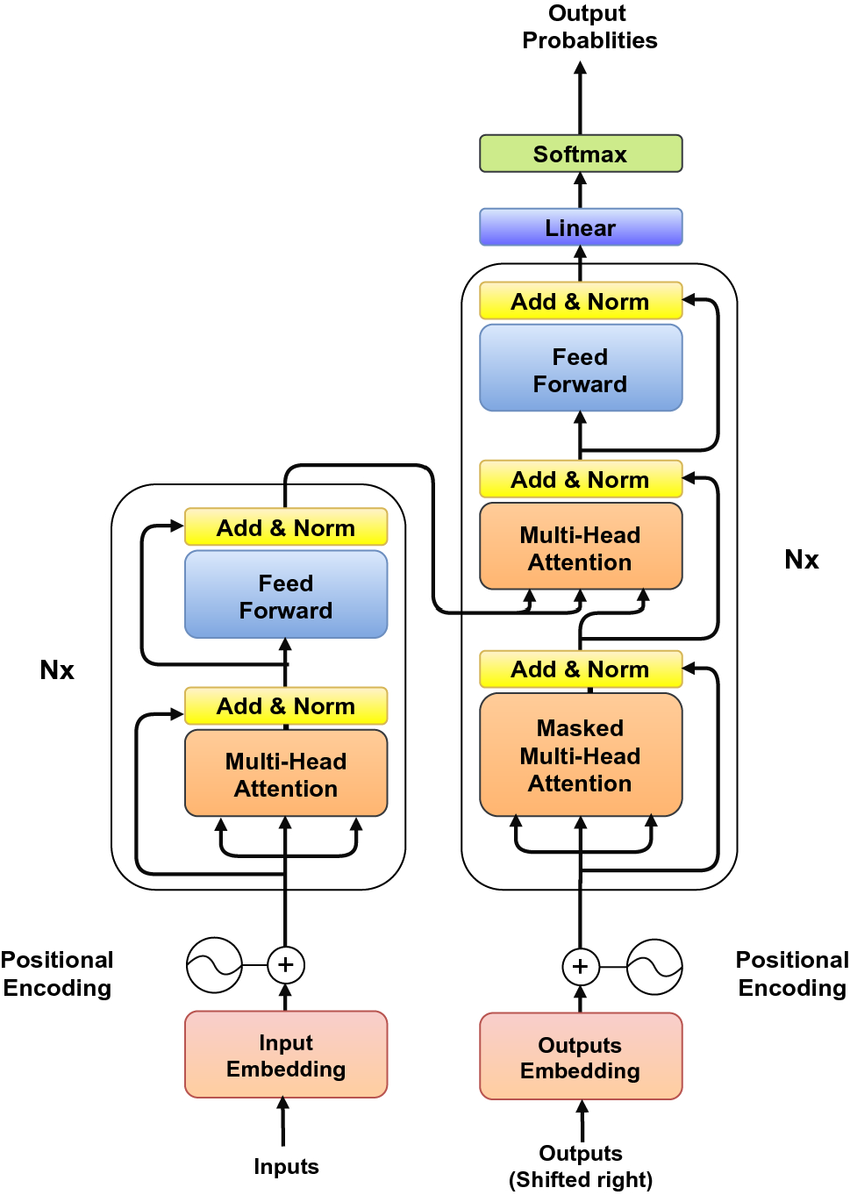
\includegraphics[width=\textwidth]{Transformer-model-architecture.png}
 		\caption{معماری ترانسفورمر ها}
 		\label{fig:transformer_architecture}
 	\end{minipage}
 	\hfill

 \end{figure}

\subsection{Embedding}
در زبان طبیعی، کلمات به شکل رشته‌های متنی هستند مانند \lr{کتاب}، \lr{ماشین} و ... . کامپیوترها نمی‌توانند به‌طور مستقیم این کلمات را به شکل رشته‌های متنی پردازش کنند. به همین دلیل، در یادگیری ماشین این کلمات را به شکل یک بردار نمایش می‌دهیم. این بردار بیانگر آن کلمه در مدل است تا ماشین بتواند آن کلمه را پردازش کند.

این بردارها ویژگی‌های کلمه را در فضای عددی نمایش می‌دهند. روش‌های مختلفی برای تبدیل متن به بردار وجود دارند. از جمله این روش‌ها می‌توان به روش‌های \lr{Word2Vec} و \lr{GloVe} اشاره کرد.

همان‌طور که در تصویر ... نشان داده شده است، هر کلمه که به صورت توکن است، ابتدا در دیکشنری تعریف‌شده پیدا می‌شود و پس از پیدا شدن در دیکشنری، با استفاده از روش‌های \lr{Embedding}، هر کلمه به برداری از اعداد تبدیل می‌شود.

این \lr{Embedding}‌ها شباهت‌های معنایی بین کلمات را مدل‌سازی می‌کنند. به‌طوری‌که کلماتی که از نظر معنایی شبیه به هم هستند، بردار آن‌ها نیز به یکدیگر نزدیک‌تر است. به این ترتیب، کلمات برای مدل‌ها و شبکه‌های عصبی قابل‌فهم می‌شوند.




 \begin{figure}[h]
	\centering
	\begin{minipage}[b]{0.7\textwidth}
		\centering
		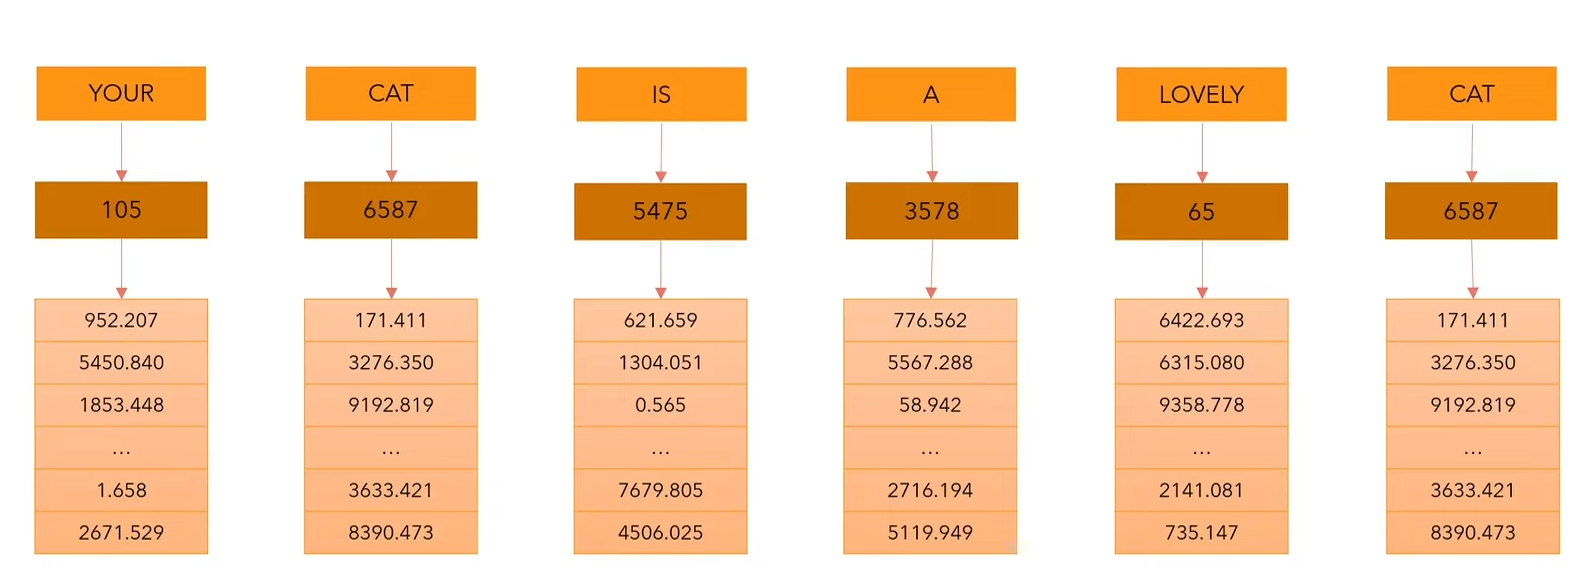
\includegraphics[width=\textwidth]{transformer_images/word_embedding.png}
		\caption{word embedding}
		\label{fig:word_embedding}
	\end{minipage}
	\hfill
	
\end{figure}



\subsection{\lr{positional embedding}}

ما تا الان هر کلمه را به برداری از اعداد که برای مدل قابل فهم باشد، تبدیل کرده‌ایم. اما مدل‌های ترانسفورمر نمی‌توانند جایگاه هر کلمه را تشخیص دهند. در مدل‌های ترانسفورمر، برخلاف مدل‌های بازگشتی، به دلیل اینکه کلمات به‌صورت موازی وارد می‌شوند، نیاز داریم تا جایگاه هر کلمه را بدانیم. به‌طور مثال، در جملهٔ من تو را دوست داریم باید به‌طور دقیق بدانیم که کلمهٔ من کلمهٔ اول جمله است، کلمهٔ تو کلمهٔ دوم جمله است و ... .

حال ما باید به مدل توالی این کلمات را بفهمانیم. بنابراین، نیاز داریم به مدل یک سری اطلاعات اضافی بدهیم به‌طوری‌که مدل توالی کلمات را یاد بگیرد. روش‌های مختلفی برای اضافه‌کردن \lr{Positional Embedding} به مدل وجود دارد. در ترانسفورمرها از روش \lr{Sinusoidal Positional Embedding} استفاده می‌شود. 

این روش قابل یادگیری نیست و صرفاً از یک سری فرمول‌های ساده برای \\lr{Positional Embedding} استفاده می‌کند.

برای موقعیت \( pos \) در توالی و بُعد \( i \) در فضای برداری، تعبیهٔ موقعیتی به‌صورت زیر تعریف می‌شود:
\[
PE(pos, 2i) = \sin\left( \frac{pos}{10000^{\frac{2i}{d}}} \right)
\]

و برای مقادیر فرد:
\[
PE(pos, 2i+1) = \cos\left( \frac{pos}{10000^{\frac{2i}{d}}} \right)
\]




\begin{figure}[h]
	\centering
	\begin{minipage}[b]{0.7\textwidth}
		\centering
		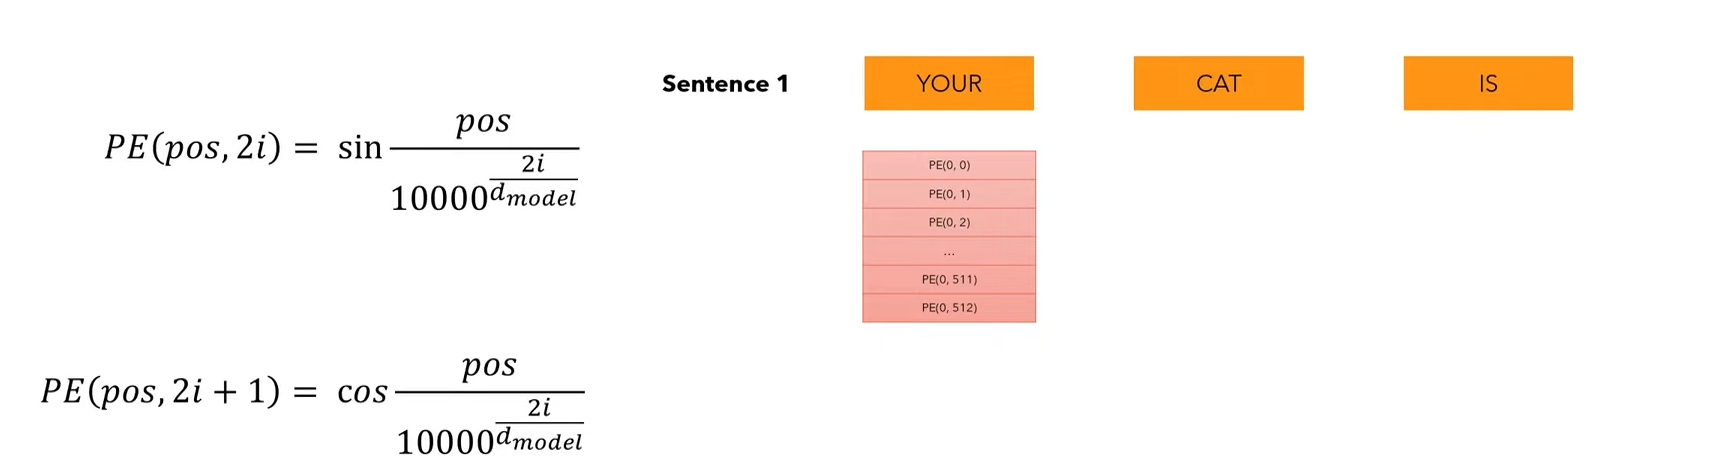
\includegraphics[width=\textwidth]{transformer_images/positional_embedding_formula .png}
		\caption{word embedding}
		\label{fig:positional embedding}
	\end{minipage}
	\hfill
	
\end{figure}



- \( pos \): موقعیت کلمه در توالی است. برای مثال، اگر توالی ورودی شامل \( N \) کلمه باشد، موقعیت‌ها از \( 0 \) تا \( N-1 \) تغییر می‌کنند. به عبارت دیگر، \( pos \) می‌تواند هر عددی از مجموعه \( \{0, 1, 2, \dots, N-1\} \) باشد که نشان‌دهنده موقعیت یک کلمه خاص در توالی است.

- \( i \): شاخص بعد در بردار موقعیتی است. این متغیر به اندیس بعدی که موقعیت کلمه در آن نمایش داده می‌شود اشاره دارد. برای مثال، اگر فضای برداری مدل دارای ابعاد \( d \) باشد، \( i \) از \( 0 \) تا \( d-1 \) تغییر می‌کند.

- \( d \): ابعاد فضای برداری مدل است. این مقدار مشخص می‌کند که هر کلمه در توالی به چه تعداد ابعاد در فضای برداری نگاشت می‌شود. به عبارت دیگر، \( d \) نشان‌دهنده تعداد ویژگی‌ها (یا ابعاد) در بردار موقعیتی است.

- \( 10000 \): یک مقدار ثابت است که برای تنظیم مقیاس توابع تناوبی استفاده می‌شود. این مقدار به‌گونه‌ای تنظیم شده است که از نوسانات زیاد جلوگیری کند و همچنین فرکانس‌های مختلفی را برای ابعاد مختلف به وجود آورد.

همانطور که در شکل زیر مشاهده میکنید بعد از \lr{embedding}  کلمات    به آن \lr{positional embedding} اضافه می شود.
که در این روش از توابع سینوس و کسینوس استفاده میشود.
این توابع موقعیت ها را در فضای برداری به گونه ای نگاشت میکنند که مدل بتواند از ترتیب کلمات در توالی آگاه باشد.این ویژگی به مدل کمک میکند تا مدل توالی زمانی را بتواند درک کند و الگو های زمانی را شبیه سازی کند.
از مزایای این مدل میتوان به عدم نیاز به آموزش و توزیع متوازن جایگاه هر کدام از کلمات اشاره کرد.


\begin{figure}[h]
	\centering
	\begin{minipage}[b]{0.7\textwidth}
		\centering
		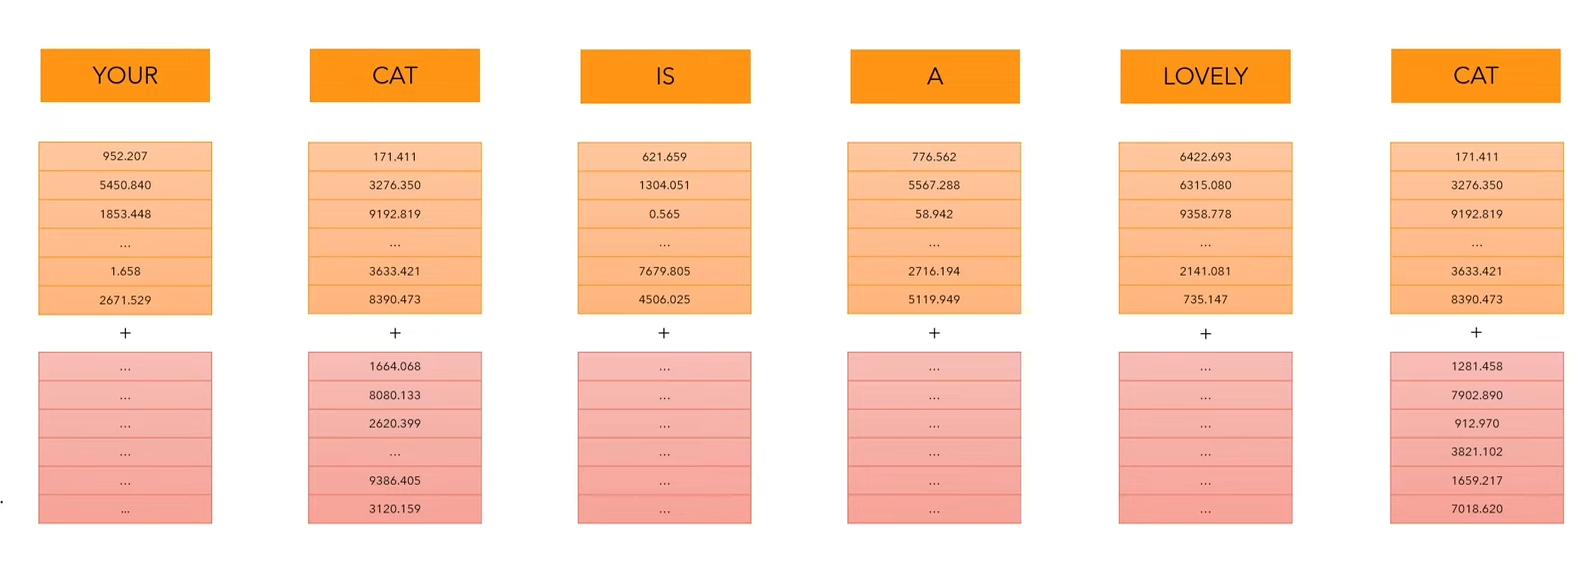
\includegraphics[width=\textwidth]{transformer_images/positional_embedding.png}
		\caption{word embedding}
		\label{fig:word embedding + positional embedding}
	\end{minipage}
	\hfill
	
\end{figure}






\subsection{attention:}



در روش‌های قدیمی (مانند RNN یا lstm)، توالی ورودی (مثلاً یک جمله) معمولاً به‌صورت گام‌به‌گام پردازش می‌شد. اما در ترانسفورمر می‌خواهیم مدلی داشته باشیم که به هر موقعیت (مثلاً یک کلمه) در توالی نگاه کند و به همهٔ موقعیت‌های دیگر نیز به‌صورت موازی دسترسی داشته باشد. به این مفهوم \textbf{توجه} می‌گوییم.
م
به زبان ساده، وقتی توکن (کلمه) $i$ به توکن‌های دیگر نگاه می‌کند، می‌خواهد بداند کدام توکن‌ها برای تفسیر معنای خودش مهم‌ترند.

به طور مثال در جمله  یک گربه روی زمین نشسته است میخواده بداند کلمه گربه به واژه نشستن بیشتر توجه کند یا به زمین، مثلا در این جا فعل نشستن ارتباط نزدیک تری به گربه دارد، و از نظر معنایی مرتبط تر است.




\[
Q = \text{Query (پرسش)}, \quad K = \text{Key (کلید)}, \quad V = \text{Value (مقدار / ارزش)}
\]

در \lr{Scaled Dot-Product Attention}، ابتدا شباهت یا ارتباط بین \lr{Query} و \lr{Key} را با محاسبهٔ ضرب داخلی (\lr{Dot Product}) به‌دست می‌آوریم، سپس آن را نرمال می‌کنیم (با تقسیم بر \( d_k \)) و از تابع \lr{softmax} استفاده می‌کنیم تا ضرایب توجه (\lr{Attention Weights}) را به‌دست آوریم. در نهایت با همین ضرایب، ترکیبی خطی از بردارهای \lr{Value} را می‌گیریم.

فرمول به‌شکل زیر است:

\[
\text{Attention}(Q, K, V) = \text{softmax}\left( \frac{QK^T}{\sqrt{d_k}} \right) V
\]

که در آن:

\[
Q \in \mathbb{R}^{n \times d_k} \quad \text{ماتریس پرسش برای} \, n \, \text{توکن}
\]
\[
K \in \mathbb{R}^{n \times d_k} \quad \text{ماتریس کلید برای} \, n \, \text{توکن}
\]
\[
V \in \mathbb{R}^{n \times d_v} \quad \text{ماتریس مقدار برای} \, n \, \text{توکن}
\]

\[
d_k \quad \text{ابعاد بردارهای پرسش و کلید است (معمولاً} \, d_k = d_{\text{model}} \, \text{در حالت چندسری)}
\]

تقسیم بر \( d_k \) باعث می‌شود مقدار ضرب داخلی در ابعاد بالا خیلی بزرگ نشود و شیب‌ها (Gradients) پایدار بمانند.

\[
\alpha = \text{softmax}\left( \frac{QK^T}{\sqrt{d_k}} \right)
\]
\(\alpha\) یک ماتریس با ابعاد \( n \times n \) است که سطر \( i \)-ام آن ضرایب توجه برای توکن \( i \) را نشان می‌دهد.

تفسیر ضرایب توجه: هر سطر از \( \alpha \) نشان می‌دهد که توکن فعلی به چه توکن‌هایی در جمله، با چه شدتی توجه می‌کند.



\begin{figure}[h]
	\centering
	\begin{minipage}[b]{0.7\textwidth}
		\centering
		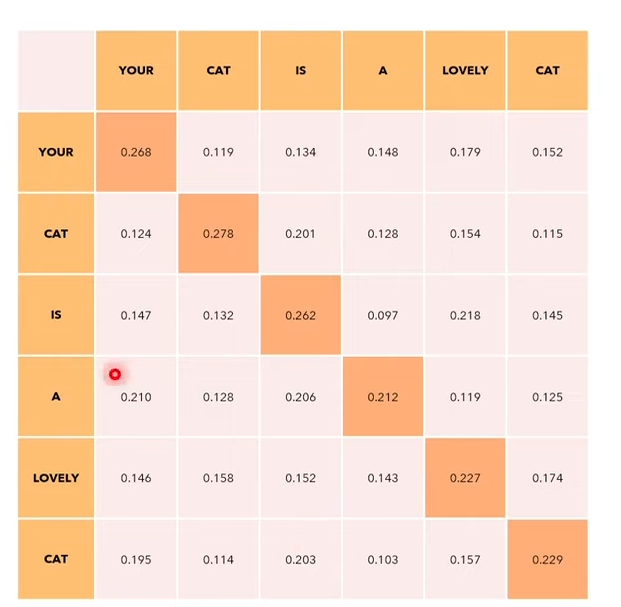
\includegraphics[width=\textwidth]{transformer_images/attention.png}
		\caption{Attention}
		\label{fig:attention}
	\end{minipage}
	\hfill
	
\end{figure}





ایدهٔ چندسری:  
به‌جای آنکه فقط یک‌بار \( Q, K, V \) بسازیم و عملیات توجه را انجام دهیم، چندین مجموعهٔ متفاوت \( Q_i, K_i, V_i \) می‌سازیم (هر کدام یک «Head» یا سر نام دارد) و به‌صورت موازی محاسبات Attention را انجام می‌دهیم. سپس خروجی همهٔ این Headها را کنار هم قرار داده (Concat) و در نهایت با یک ماتریس وزن دیگر ضرب می‌کنیم تا به بعد اصلی بازگردیم.

فرمول مربوط به این ایده به‌شکل زیر است:

\[
\text{head}_i = \text{Attention}(Q_i, K_i, V_i)
\]
\[
\text{MultiHead}(Q, K, V) = [\text{head}_1 \oplus \cdots \oplus \text{head}_h] W_O
\]

که در آن \( \oplus \) نشان‌دهندهٔ عمل الحاق (Concatenation) است.

ماتریس وزن \( W_O \) به‌شکل زیر است:

\[
W_O \in \mathbb{R}^{(h \cdot d_v) \times d_{\text{model}}}
\]

که \( W_O \) ماتریسی است که خروجی الحاق‌شده را به بعد \( d_{\text{model}} \) برمی‌گرداند.





\begin{figure}[h]
	\centering
	\begin{minipage}[b]{0.9\textwidth}
		\centering
		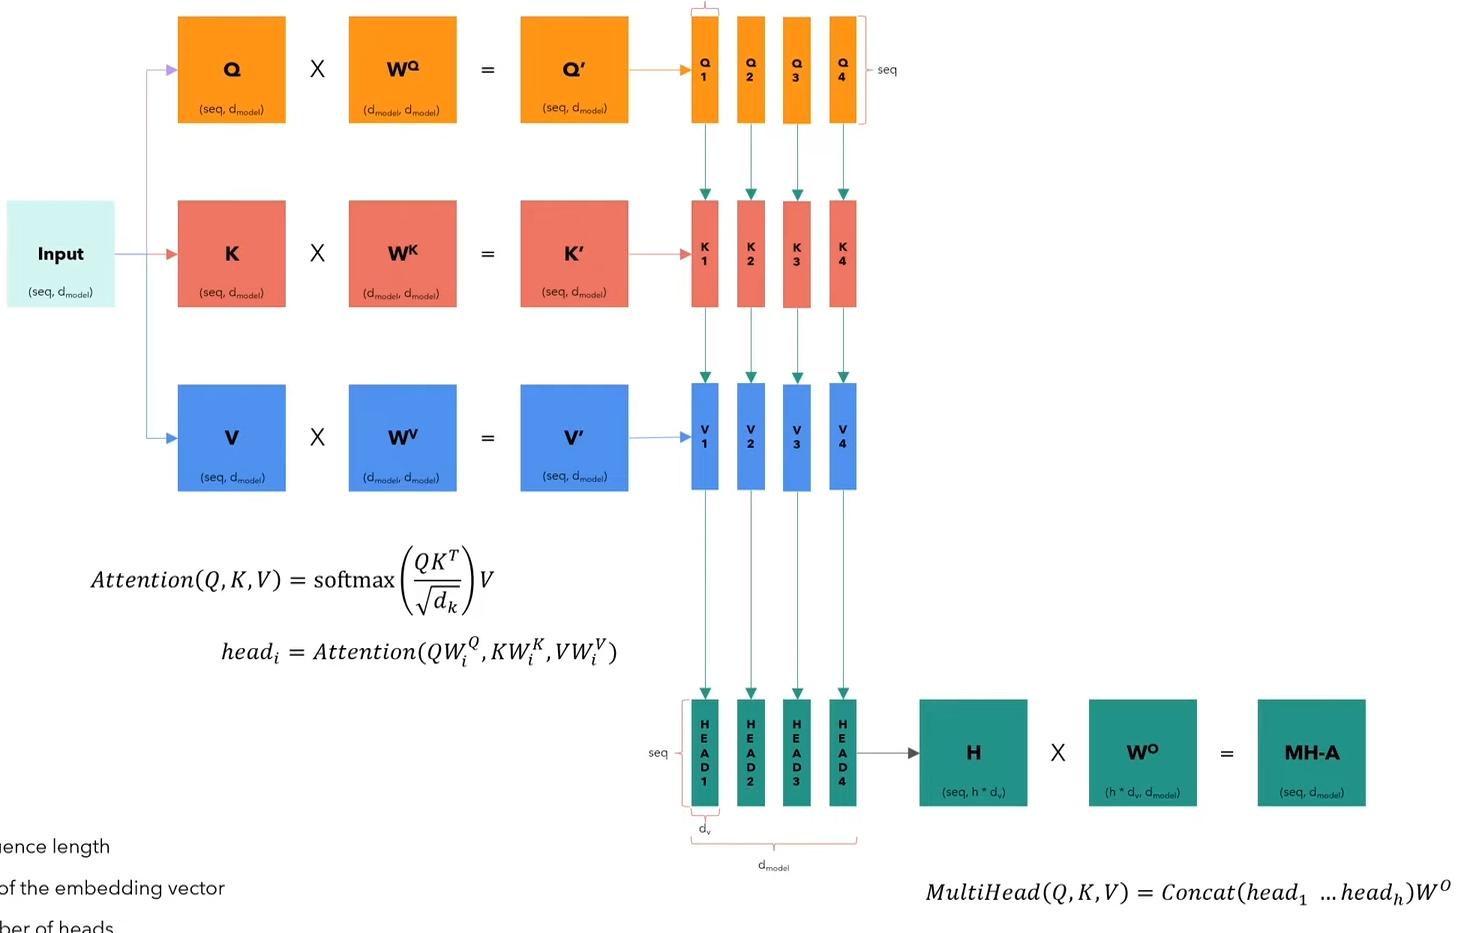
\includegraphics[width=\textwidth]{transformer_images/multi_head_attention.png}
		\caption{\lr{multi head attention}}
		\label{fig:attention}
	\end{minipage}
	\hfill
	
\end{figure}



\subsection*{چرا چندین سر؟}

\textbf{مشاهدهٔ چند منظر متفاوت:} هر Head می‌تواند الگوهای گوناگونی از وابستگی‌ها را بیاموزد (مثلاً یک Head می‌تواند یاد بگیرد کلمهٔ فعلی با کلمات همسایهٔ نزدیک خود بیشتر مرتبط شود، یک Head دیگر روی ارتباط با کلماتی در فاصلهٔ دورتری متمرکز باشد، Head دیگر روی مطابقت جنس و تعداد در دستور زبان و ...).

\textbf{افزایش ظرفیت مدل:} با داشتن چند Head، مدل می‌تواند قدرت بیان بیشتری داشته باشد.

\textbf{ابعاد کمتر در هر Head:} در عمل، اگر \( d_{\text{model}} \) مثلاً 512 باشد، و تعداد Headها \( h = 8 \)، آنگاه هر Head ابعادی در حدود \( d_k = 64 \) خواهد داشت؛ و این محاسبات ضرب داخلی را نیز مقیاس‌پذیر و قابل موازی‌سازی می‌کند.


\subsection{\lr{Residual Connection (Add)}}
در معماری های های مختلف هنگامی که تعداد لایه ها زیاد  میشود، اغلب دچار ناپایداری گرادیان (\lr{Vanishing/Exploding Gradients}) میشوند. و باعث مشکل در آموزش مدل میشود.
در مدل ترانسفورمر به جای این که خروجی \lr{attention}  را به صورت مستقیم به لایه بعدی بدهیم، ورودی آن را نیز حفظ کرده و به خروجی اضافه میکنیم.
اگر \( x \) ورودی به زیرماژول و \( \text{SubLayer}(x) \) خروجی آن زیرماژول باشد، در انتهای کار، ما عبارت زیر را محاسبه می‌کنیم:


\[
x + \text{SubLayer}(x)
\]

این جمع به صورت عنصر به عنصر (\lr{Element-wise Addition})  انجام میشود.


\subsection{مزایای \lr{Residual Connection} در ترانسفورمر}

\subsection*{کمک به جریان یافتن گرادیان}

وقتی ورودی مستقیماً به خروجی اضافه می‌شود، مسیری مستقیم برای عبور شیب (گرادیان) به عقب ایجاد می‌گردد.
در صورت نبود این اتصال، اگر شبکه عمیق شود، گرادیان‌ها ممکن است در لایه‌های پایین محو شوندو عملا \lr{gradient vanishing} رخ میدهد.

\subsection*{حفظ اطلاعات اصلی (هویت ورودی)}

حتی اگر زیرماژول تغییری در اطلاعات ورودی ایجاد کند، با وجود \lr{Residual Connection}، ورودی اصلی همواره در خروجی نهایی حضور دارد.
این ویژگی باعث می‌شود در صورت ناکافی بودن یادگیری زیرماژول یا در مراحل اولیهٔ آموزش، دست‌کم بخشی از سیگنال/اطلاعات خام به لایه‌های بالاتر برسد.

\subsection*{کاهش ریسک تخریب ویژگی‌ها}

در شبکه‌های عمیق، یکی از مشکلات این است که هر لایه ممکن است بخشی از اطلاعات مفید را تخریب کند. \lr{Residual Connection} تضمین می‌کند که اگر لایه‌ای به هر دلیل نتوانست الگوی بهینه را یاد بگیرد، اطلاعات قبلی حداقل به صورت دست‌نخورده تا حدی منتقل می‌شود.

\section{Layer Normalization (Norm):}

در یادگیری عمیق، نرمال‌سازی (Normalization) داده‌های یک لایه یا فعال‌سازی‌ها، اغلب به سرعت بخشیدن به همگرایی و پایدار کردن آموزش کمک شایانی می‌کند. شاید معروف‌ترین نوع نرمال‌سازی، \lr{Batch Normalization} باشد که پیش‌تر در کارهای بینایی (CNNها) بسیار مورداستفاده قرار گرفت.

\lr{Layer Normalization} روشی جایگزین است که در ترانسفورمر استفاده می‌شود. علت اصلی این انتخاب، ماهیت توالی‌محور (Sequence) بودن داده‌ها در NLP و عدم تمایل به وابستگی به آمار مینی‌بچ است.



\subsection*{تفاوت \lr{Layer Norm} با \lr{Batch Norm}}

\subsection*{\lr{Batch Normalization}}

در \lr{Batch Norm}، برای نرمال‌سازی، میانگین و واریانس روی تمام نمونه‌های موجود در مینی‌بچ (و نیز در طول ابعاد ویژگی) محاسبه می‌شود.
این موضوع در NLP کمی دردسرساز است؛ چون ترتیب (Order) توکن‌ها، طول جمله‌ها و حتی اندازهٔ مینی‌بچ ممکن است نامنظم باشد.
همچنین به خاطر تنوع طول توالی‌ها (\lr{Sequence Length})، پیاده‌سازی \lr{Batch Norm} می‌تواند پیچیده شود.

\subsection*{\lr{Layer Normalization}:}

در \lr{Layer Norm،} برای هر توکن به‌صورت جداگانه (در طول بُعد ویژگی)، میانگین و واریانس گرفته می‌شود.
فرض کنید در یک لایه، بردار \( h_i \in \mathbb{R}^{d_{\text{model}}} \) مربوط به توکن \( i \) باشد؛ یعنی ابعاد ویژگی آن \( d_{\text{model}} \) است. ما میانگین \( \mu_i \) و واریانس \( \sigma_i^2 \) را از اجزای این بردار محاسبه می‌کنیم:

\[
\mu_i = \frac{1}{d_{\text{model}}} \sum_{k=1}^{d_{\text{model}}} h_{i,k}, \quad
\sigma_i^2 = \frac{1}{d_{\text{model}}} \sum_{k=1}^{d_{\text{model}}} (h_{i,k} - \mu_i)^2
\]

سپس نرمال‌سازی برای هر مؤلفهٔ \( k \) در بردار توکن \( i \) به شکل زیر انجام می‌شود:

\[
\hat{h}_{i,k} = \frac{h_{i,k} - \mu_i}{\sqrt{\sigma_i^2 + \epsilon}}
\]

در نهایت، برای این‌که مدل بتواند مقیاس و بایاس جدیدی یاد بگیرد، شبیه  ,\lr{Batch Norm}، دو پارامتر \( \gamma \) (Scale) و \( \beta \) (Bias) نیز در طول بعد ویژگی اعمال می‌شوند:

\[
\text{LayerNorm}(h_i) = \gamma \odot \hat{h}_i + \beta
\]

که در آن \( \gamma, \beta \in \mathbb{R}^{d_{\text{model}}} \) هستند و \( \odot \) ضرب عنصر به عنصر است.

\subsection*{مزایای \lr{Layer Normalization} در ترانسفورمر}

\begin{itemize}
	\item \textbf{بی‌نیازی از وابستگی به ابعاد مینی‌بچ:}  
	با Layer Norm، می‌توان حتی با اندازهٔ مینی‌بچ برابر ۱ نیز به‌خوبی آموزش دید، چراکه آمارها وابسته به ابعاد ویژگی‌اند و نه مینی‌بچ.
	
	\item \textbf{پایدارسازی توزیع فعال‌سازی‌ها:}  
	زمانی که مدل در حال یادگیری است، توزیع‌های داخلی لایه‌های میانی ممکن است تغییر کند (پدیدهٔ \lr{Internal Covariate Shift}). \lr{Layer Norm } با نرمال ‌سازی این توزیع، آموزش را پایدارتر و سریع‌تر می‌کند.
	
	\item \textbf{سازگاری با داده‌های توالی‌محور:}  
	هر توکن را جداگانه نرمال می‌کند و نگرانی‌ای بابت ترتیب طول جمله‌ها، یا قرار گرفتن چند جملهٔ کوتاه/بلند در یک مینی‌بچ نداریم.
\end{itemize}





در معماری ترانسفورمر، پس از خروجیِ هر زیرماژول (مثل Attention یا MLP)، مراحل به‌شکل زیر است:

\lr{Residual Connection:} ابتدا ورودی همان زیرماژول (مثلاً بردار \( x \)) را با خروجی زیرماژول (\( \text{SubLayer}(x) \)) جمع می‌کنیم. حاصل این جمع را می‌توان چنین نوشت:

\[
z = x + \text{SubLayer}(x)
\]

این \( z \) حالا ترکیبی از اطلاعات اصلی ورودی و اطلاعات یادگرفته‌شده توسط SubLayer است.

\lr{Layer Normalization:} سپس این بردار \( z \) را وارد لایهٔ \text{LayerNorm} می‌کنیم:

\[
y = \text{LayerNorm}(z)
\]

خروجی نهایی را می‌توان به لایهٔ بعدی پاس داد یا به مرحلهٔ بعدی در همین لایه.

به‌عبارتی اگر بخواهیم در یک فرمول واحد بیان کنیم:

\[
\text{Add \& Norm} = \text{LayerNorm}\left(x + \text{SubLayer}(x)\right)
\]

\section{\lr{decoder}}

دیکودر  در معماری ترانسفورمرها وظیفه تولید خروجی نهایی را بر عهده دارد. این خروجی معمولاً می‌تواند توالی هدف (Target Sequence) باشد، مثل ترجمه یک جمله یا پیش‌بینی توکن‌های بعدی در یک توالی.
در ابن بخش دیکدر دو ورودی اصلی دارد:
 توالی هدف که معمولاً به صورت خودکار تولید می‌شود (مثلاً در ترجمه ماشینی یا تولید متن)، و نمایش (Representation) کدشده که توسط انکودر (Encoder) تولید شده است و شامل ویژگی‌های استخراج‌شده از توالی ورودی می‌باشد. دیکودر از این ورودی‌ها استفاده می‌کند تا به صورت گام‌به‌گام، خروجی نهایی خود را تولید کند.
 
 
 همانطور که در تصویر مشاهده میکنید دیکدر دو ورودی دارد.
 

\begin{figure}[h]
	\centering
	\begin{minipage}[b]{0.25\textwidth}
		\centering
		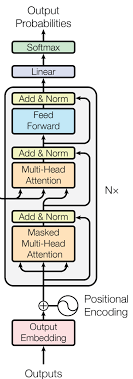
\includegraphics[width=\textwidth]{transformer_images/decoder.png}
		\caption{Decoder}
		\label{fig:Decoder}
	\end{minipage}
	\hfill
	
\end{figure}

تمامی بخش های دیکدر مانند انکدر میباشند اما در دیکدر masked multi head attention  وجود دارد.

\section{masked multi head attention}


در ترانسفورمر، مکانیزم Multi-Head Attention در بخش دیکودر به‌صورت Masked پیاده‌سازی می‌شود تا مدل نتواند توکن‌های آینده را ببیند و به‌صورت خودبازگشتی (Autoregressive) توکن بعدی را پیش‌بینی کند.
در واقع ایده اصلی استفاده از mask  جلوگیری از مشاهده آینده است.




 در معماری‌های خودبازگشتی (\textit{Autoregressive})، مدل در گام \( i \) از دیکودر تنها باید به توکن‌های قبلی \( \{ y_1, \dots, y_{i-1} \} \) دسترسی داشته باشد؛ اما نه به توکن‌های \( \{ y_{i+1}, y_{i+2}, \dots \} \). اگر مدل بتواند توکن‌های آینده را «نگاه» کند، پیش‌بینی توکن بعدی آسان و غیرواقعی می‌شود (مشکل نشت اطلاعات).
 
 به همین دلیل در \textit{Masked Multi-Head Self-Attention} دیکودر، از یک ماتریس ماسک \( M \) استفاده می‌کنیم که اجازه نمی‌دهد هر توکن به توکن‌های آینده‌اش توجه کند.
 
 \section{مثال عددی mask attention:}
 
 فرض کنید دنبالهٔ 4 توکنی داریم:
 \[
 [y_1, y_2, y_3, y_4]
 \]
 خروجی Scaled Dot-Product (قبل از \texttt{softmax}) یک ماتریس \( 4 \times 4 \) خواهد بود:
 \[
 S =
 \begin{bmatrix}
 	s_{1,1} & s_{1,2} & s_{1,3} & s_{1,4} \\
 	s_{2,1} & s_{2,2} & s_{2,3} & s_{2,4} \\
 	s_{3,1} & s_{3,2} & s_{3,3} & s_{3,4} \\
 	s_{4,1} & s_{4,2} & s_{4,3} & s_{4,4}
 \end{bmatrix}
 \]
 
 برای سطر 1 (توکن اول): می‌تواند خودش (ستون 1) را ببیند، اما ستون‌های 2 تا 4 را ماسک می‌کنیم.
 برای سطر 2 (توکن دوم): می‌تواند به ستون‌های 1 و 2 نگاه کند، اما 3 و 4 ماسک می‌شوند.
 برای سطر 3: ستون‌های 1، 2 و 3 را ببیند، ستون 4 ممنوع است.
 برای سطر 4: ستون 1، 2، 3، 4 آزاد است. (چون چهارمین توکن می‌تواند توکن‌های قبلی را ببیند، و از طرفی این توکن «خودش» نیز موردی ندارد - بسته به پیاده‌سازی ممکن است تصمیم بگیریم توکن فعلی از خودش نیز استفاده کند یا نه؛ در معماری استاندارد، سطر \( i \) معمولاً به ستون \( i \) هم دسترسی دارد.)
 
 در عمل، ماتریس ماسک \( M \) به شکل زیر خواهد بود (اگر به شکل پایین‌مثلثی نشانه‌گذاری کنیم):
 \[
 M =
 \begin{bmatrix}
 	0 & -\infty & -\infty & -\infty \\
 	0 & 0 & -\infty & -\infty \\
 	0 & 0 & 0 & -\infty \\
 	0 & 0 & 0 & 0
 \end{bmatrix}
 \]
 
 به این ترتیب، پس از جمع شدن با \( S \) و اجرای \texttt{softmax} در هر سطر، ضرایب توجه‌ی ستون‌های ماسک‌شده به صفر میل می‌کنند.
 
 
 
 
 \section{vision transformer:}

ایده ترانسفورمر ها در تصویر از تعمیم دادن ترانسفومر متن به وجود آمده است.

 
 ما در این بخش vision transformer را در کلاس بندی استفاده میکنیم.
 
 در روش های متداول برای پردازش تصویر از convolution  ها استفاده می کردند.
 اما در ترانسفورمر ها عکس ها به پج های مختلف شکسته می شوند.
 و این قسمت های شکسته شده عکس به یک دیگر توجه میکنند که  چقدر به یک دیگر شباهت دارند.
 در قسمت های بعد به طور مفصل به این کار ها میپردازیم.
 
 \subsection{patch embedding in vision transformer:}
 
 
 
در ترانسفورمر های مبتنی بر متن هر کلمه به توکن تبدیل می شود. و هر کدام از این کلمات به بردار هایی تبدیل میشود. و  این بردار ها بعد از اضافه شده positional embedding وارد Attention  در ترانسفورمر ها میرسید.

حال همین ایده در تصویر پیاده سازی شده است.
همانطور که در تصویر ... مشاهده  می کنید. 

 در Vision Transformer، به‌جای عملیات کانولوشن، مستقیماً تصویر را به بلاک‌های غیرهم‌پوشان ($P \times P$) قطعه‌بندی می‌کنیم تا موازی‌سازی بهتری داشته باشیم و به مدل اجازه دهیم از سازوکار Self-Attention (توجه سراسری) برای ارتباط بین این بلاک‌ها استفاده کند.




\begin{figure}[h]
	\centering
	\begin{minipage}[b]{0.9\textwidth}
		\centering
		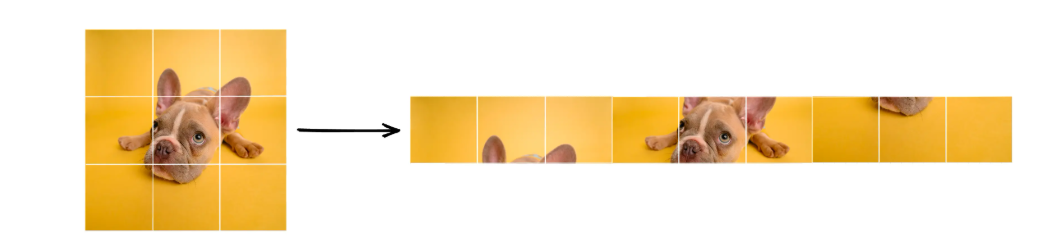
\includegraphics[width=\textwidth]{transformer_images/image_patch_embedding.png}
		\caption{iamge to patch}
		\label{fig:image to patch in vision transformer}
	\end{minipage}
	\hfill
	
\end{figure}


\subsection{شکل پچ ها:}

فرض کنید ابعاد تصویر ورودی ($H \times W \times C$) است. به‌عنوان مثال:


فرض کنیم اندازه تصویر ما $224 \times 224 \times 3$ باشد. یعنی طول و عرض تصویر به ترتیب 224 و سه کانال رنگی داشته باشد.
\[
H = 224, \quad W = 224, \quad C = 3
\]




\begin{figure}[h]
	\centering
	\begin{minipage}[b]{0.9\textwidth}
		\centering
		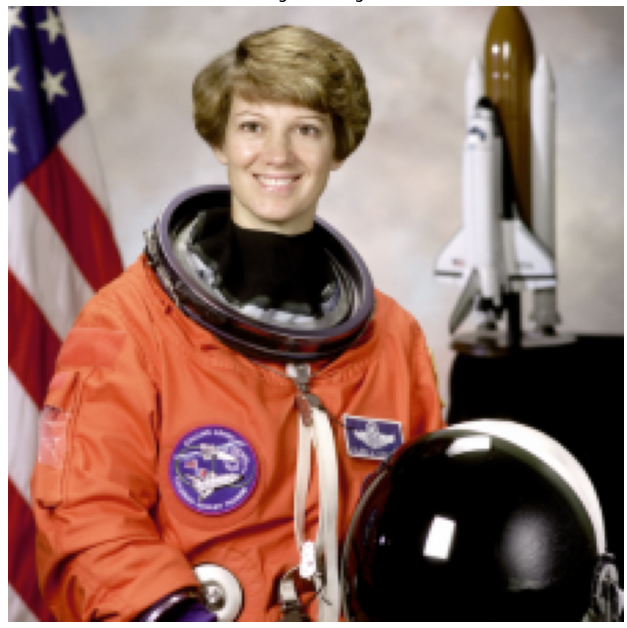
\includegraphics[width=\textwidth]{transformer_images/space_original_image.png}
		\caption{original Image}
		\label{fig:Original Image}
	\end{minipage}
	\hfill
	
\end{figure}


حال اگر اندازهٔ هر پچ ($P \times P$) باشد (مثلاً $16 \times 16$)، تصویر به‌صورت یک جدول مشبک از پچ‌های کوچک تقسیم می‌شود.

به هر پچ می‌توان مانند یک «کاشی» از تصویر نگاه کرد:
پچ اول: مختصات (0 تا 15 در ارتفاع) و (0 تا 15 در عرض)،
پچ دوم: مختصات (0 تا 15 در ارتفاع) و (16 تا 31 در عرض)،
و به همین ترتیب تا کل تصویر پوشش داده شود.



\begin{figure}[h]
	\centering
	\begin{minipage}[b]{0.9\textwidth}
		\centering
		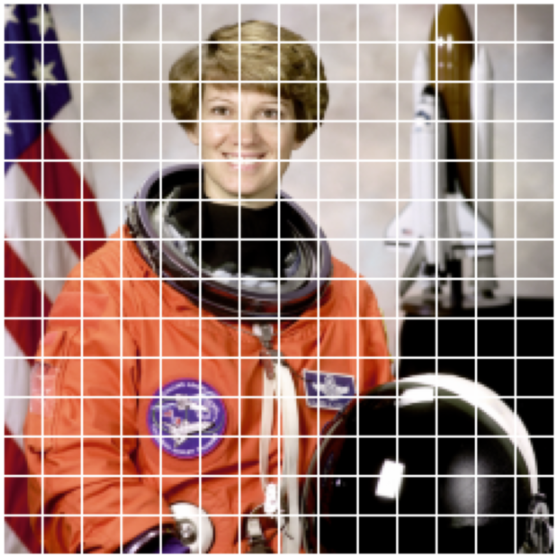
\includegraphics[width=\textwidth]{transformer_images/space_patch_iamge.png}
		\caption{patch Image}
		\label{fig:Patch Image}
	\end{minipage}
	\hfill
	
\end{figure}

\subsection{تعداد پچ ها:}

اگر پچ‌های ما بدون هم‌پوشانی باشند، ابعاد پچ دقیقاً باید بر ابعاد تصویر بخش‌پذیر باشد.


تعداد پچ‌ها افقی:
\[
\frac{W}{P}
\]
تعداد پچ‌ها عمودی:
\[
\frac{H}{P}
\]
در مجموع:
\[
\left(\frac{H}{P}\right) \times \left(\frac{W}{P}\right) = \frac{H}{P} \times \frac{W}{P}.
\]

برای مثال اگر:
\[
H = 224, \quad W = 224, \quad P = 16:
\]
\[
\frac{224}{16} = 14 \quad \Rightarrow \quad 14 \times 14 = 196 \quad \text{(تعداد پچ‌ها)}.
\]

ئر اکثر نسخ های مبدل های بینایی، چ ها بدون هم پوشانی هستند.(Non-overlapping)
اندازه پچ های کوچک باعث می شود، تعداد پچ ها زیاد شوند. و با زیاد شدن تعداد پچ ها، هزینه attention  زیاد میشود. و هم چنین اندازه پچ های بزرگ باعث میشود تعداد پچ ها کمتر شود، و هزینه های attention کمتر شود. اما در پچ های بزرگ باعث میشود که جزییات محلی (local) از بین برود.

\subsection{بردار کردن هر پچ}

هر پچ دارای ابعاد \((P \times P \times C)\) است. برای مثال اگر \(P = 16\) و \(C = 3\)، پچ ابعاد \(16 \times 16 \times 3\) دارد.
برای این‌که بتوانیم پچ‌ها را مانند «توکن»‌های NLP به مدل ترانسفورمر بدهیم، باید آن‌ها را به یک بردار یک‌بعدی تبدیل کنیم.
اگر بخواهیم همهٔ پیکسل‌های پچ را به‌صورت ردیفی (Row-major) دنبال هم بگذاریم، طول این بردار خواهد بود:
\[
P \times P \times C = P^2 \times C.
\]
در مثال \(16 \times 16 \times 3\)، طول بردار می‌شود \(768\).

\section{اعمال لایهٔ خطی (Projection):}


بعد از Flatten کردن، معمولاً یک لایهٔ خطی (Fully-Connected Layer) روی این بردار اعمال می‌شود تا آن را به بعد \(d_{\text{model}}\) (مثلاً 768 یا 1024) ببرد.
در حقیقت، این لایه تبدیل  (Feature Transformation) را  انجام می‌دهد تا همهٔ پچ‌ها یک نمایندگی (Embedding) با ابعاد یکنواخت \(d_{\text{model}}\) پیدا کنند:
\[
(P^2 \times C) \quad \rightarrow \quad d_{\text{model}}.
\]



\begin{figure}[h]
	\centering
	\begin{minipage}[b]{0.9\textwidth}
		\centering
		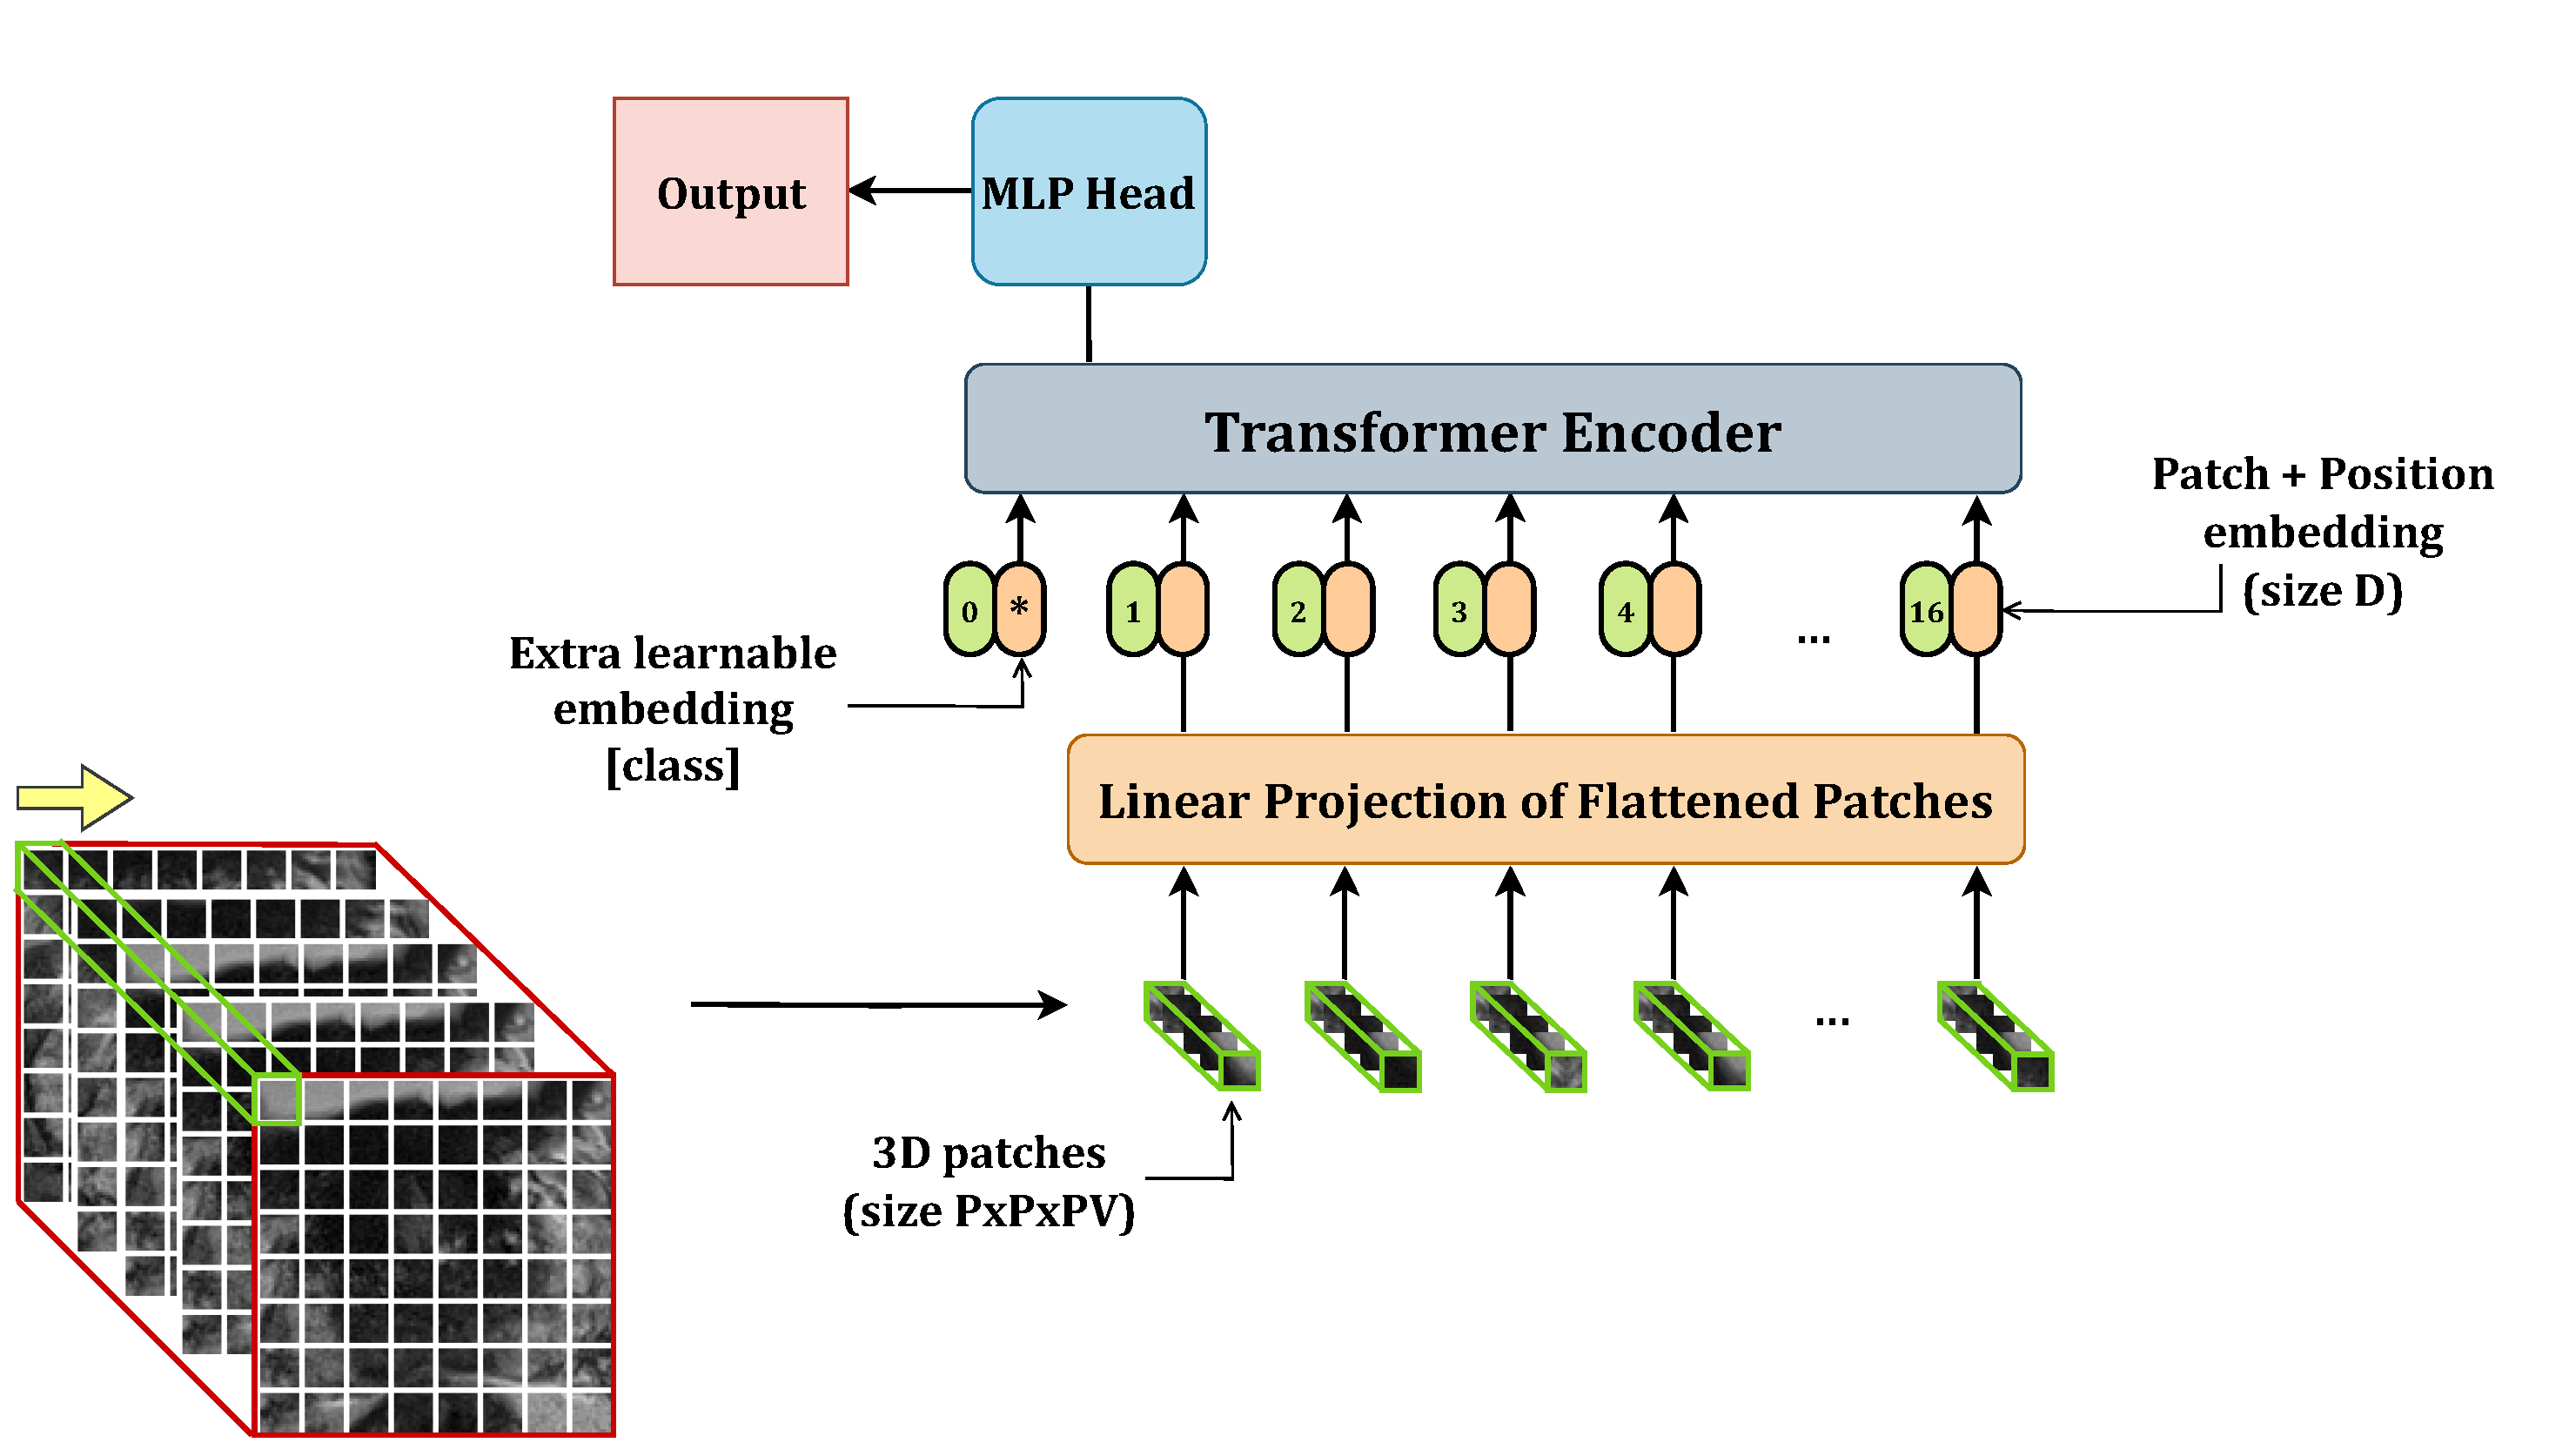
\includegraphics[width=\textwidth]{transformer_images/vision_transformer_embedding.png}
		\caption{Embedding in Vision Transformer}
		\label{fig:Embedding Vision Transformer}
	\end{minipage}
	\hfill
	
\end{figure}




این مرحله شبیه ساخت توکن در NLP است؛ با این تفاوت که در NLP توکن «کلمه» یا «زیرکلمه» است و پیش‌تر دارای بردار تعبیه‌شده Embedding شده بوده است. در vision transformer  ما ابتدا باید تصاویر را پچ کنیم و سپس بردار های embedding  شده را از این پچ ها به دست آوریم. 

ترانسفورمر نیاز دارد ورودی‌اش توالی توکن‌ها باشد. در NLP توالی کلمات داریم، در ViT توالی «پچ»‌ها:
\[
\{ x_{\text{patch}_1}, x_{\text{patch}_2}, \dots, x_{\text{patch}_N} \}.
\]
هر پچ اکنون یک بردار \(d_{\text{model}}\)-بعدی است. پس یک مجموعه با طول \(N\) (تعداد پچ‌ها) و عرض \(d_{\text{model}}\) خواهیم داشت.
اگر عدد پچ‌ها \(N\) باشد (مثلاً 196)، ترانسفورمر می‌تواند خودش با استفاده از مکانیزم Self-Attention، وابستگی (Relations) میان پچ‌ها را یاد بگیرد: کدام بخش از تصویر برای کدام بخش دیگر مهم‌تر است، چگونه ترکیب جهانی (Global Context) ساخته شود، و غیره.


معمولاً پچ‌ها را به‌صورت ردیفی (Row by Row) شماره‌گذاری می‌کنند (ابتدا پچ‌های ردیف بالایی از چپ به راست، سپس ردیف بعدی و …)، تا مدل در صورت نیاز بتواند از پوزیشن‌ها اطلاعات مکانی تقریبی داشته باشد.
در عمل، چون قصد داریم (در مراحل بعد) به هر پچ یک Positional Embedding هم اضافه کنیم، مکان دقیق هر پچ در بعد دوم (ویژگی) رمز می‌شود.

در ویژن ترانسفورمر دیگر به کانولوشن وابسته نیست.
در عوض از embedding  استفاده میشود.

Split کردن تصویر به بلاک‌های \((P \times P)\)، Flatten و Linear Projection، عملیات ریاضی ساده‌ای هستند و به راحتی قابل موازی‌سازی روی GPU/TPU هستند.


\subsection{CLS Token:}

CLS Token یک بردار ویژه است که به ابتدای دنبالهٔ ورودی اضافه می‌شود و نقش آن این است که اطلاعات کلی و مرتبط با دنبالهٔ ورودی (چه متن، چه تصویر) را در خود خلاصه کند.  
cls token 


در به ابتدای پج های تصویری قرار میگیرد.

   این توکن یک بردار با ابعاد $d_{\text{model}}$ است (همان ابعاد سایر توکن‌ها).
   
        بردار CLS یک پارامتر یادگرفتنی است، یعنی مدل در طول آموزش مقادیر آن را برای ذخیره و تجمیع اطلاعات بهینه می‌کند.
   


در وظایف دسته‌بندی (Classification)، هدف اصلی این است که یک پیش‌بینی کلی برای کل ورودی (مثلاً یک جمله یا یک تصویر) ارائه دهیم. CLS Token دقیقاً همین وظیفه را بر عهده دارد.


CLS Token 
از طریق مکانیزم \textit{Self-Attention} در ترانسفورمر می‌تواند با همهٔ توکن‌های دیگر (یعنی پچ‌های تصویر) ارتباط برقرار کند و اطلاعات مهم آن‌ها را در طول لایه‌های ترانسفورمر به‌صورت تدریجی یاد بگیرد. و به عنوان نماینده ای از تمام تصویر یا متن ها در مدل خضور پیدا کند.

     CLS Token از طریق ضرب داخلی در مکانیزم Attention می‌تواند به تمام پچ‌ها نگاه کند. ضرایب توجه ($\alpha$) تعیین می‌کند که CLS Token چه مقدار اطلاعات از هر پچ دریافت کند.

و چقدر در پروسه مدل دخیل باشد.

     CLS Token به‌طور ضمنی یاد می‌گیرد که روی ویژگی‌هایی که برای دسته‌بندی مهم هستند (مانند الگوها، اشکال و بخش‌های کلیدی تصویر) تمرکز کند.


    در طول لایه‌های ترانسفورمر، CLS Token نقش محوری در تنظیم بازنمایی کل تصویر ایفا می‌کند. به عبارت دیگر، این توکن به نوعی مرکز پردازش کل اطلاعات تصویر است.
    
    

   cls Token 
   به عنوان پارامتر های یادگیرنده تعریف میشود و این پارامتر ها در طول فرایند یادگیری بروز رسانی میشوند.
   
   \subsection{vision transformer encoder:}
   
  
  انکودر در ترانسفورمر ها همانطور که مشاهده می کنید به مانند ترانسفورمر  اصلی است در اخر با این تفاوت که دیگر به دیکدر نمیرویم و پس از عبور از بلاک های ترانسفورمر در ساده ترین حالت یک لایه خطی (Fully Connected) یا یک لایه Mlp (Multi-Layer Perceptron)
   روی بردار نهایی اعمال می شود و این لایه ها به تعداد کلاس ها خروچی میدهد.
   سپس خروجی هر لایه با گذر از تابع softmax  به احتمال هر کلاس تبدیل می شود.
   و در نهایت مدل کلاس با بیشترین احتمال را به عنوان خروجی پیش بینی میکند.
   
   
   
       \begin{figure}[h]
   	\centering
   	\begin{minipage}[b]{0.9\textwidth}
   		\centering
   		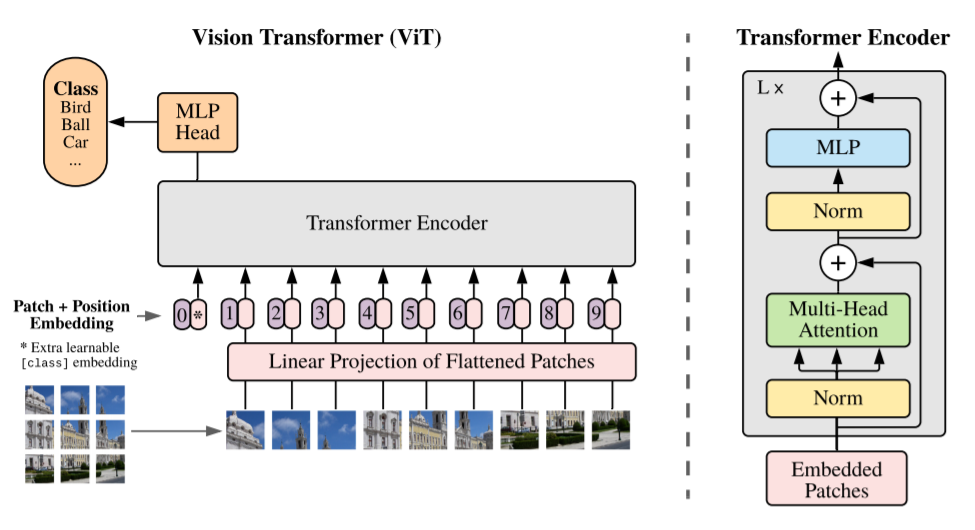
\includegraphics[width=\textwidth]{transformer_images/vision_transformer_after_embedding.png}
   		\caption{Cls Token in Vision Transformer}
   		\label{fig:Cls Token In Vision Transformer}
   	\end{minipage}
   	\hfill
   	
   \end{figure}
   
   
   در ترانسفورمر ها، هر لایه انکودر و دیکودر با پردازش عمیق تری روی توالی ورودی میتواند نمایش بهتری از ویژگی ها را به دست بیاورد.
   تکرار چندین باره encoder  یا Decoder باعث میشود مدل بتواند ساختار های پیچیده ای را یاد بگیرد و کیفیت و دقت مدل در شناسایی توالی های طولانی و معنا های پنهان افزایش یاید . در نتیجه مدل با تعداد لایه های بیشتر اغلب عملکرد بهتری از خود نشان میدهد.
   
   
   
\section{Swin Transformer:}

ایده swin transformer  از ترکیب چند مفهوم کلیدی در مدل های ترانسفورمر و شبکه های کانولوشنی شکل گرفت.
یکی از بزرگترین مشکلات در ترانسفورمر های اولیه، نیاز به محاسبات بسیار زیاد در زمانی بود که تصویر ورودی تبعاد بسیار بزرگی داشت.
در ترانسفورمر معمولی هر پچ به تمامی پچ های دیگر توجه (attention) میکرد.

و در مواقعی که تعداد پچ ها زیاد میشد، هزینه محاسباتی و حافظه به شدت افزایش پیدا میکرد.

در شبکه های کانولوشنی، معماری معمولا به صورت سلسه مراتبی پیش می رود.
یعنی ابتدا ویژگی های محلی استخراج میشود، سپس با عمیق تر شدن لایه ها، این ویژگی در سطوح بالا با یک دیگر ترکیب میشوند. در Swin transformer  با دانش بر این موضوع، میتوانند هم هزینه های محاسباتی را کاهش دهند و هم دقت مدل را افزایش دهند.

 
   
\begin{figure}[h]
	\centering
	\begin{minipage}[b]{1\textwidth}
		\centering
		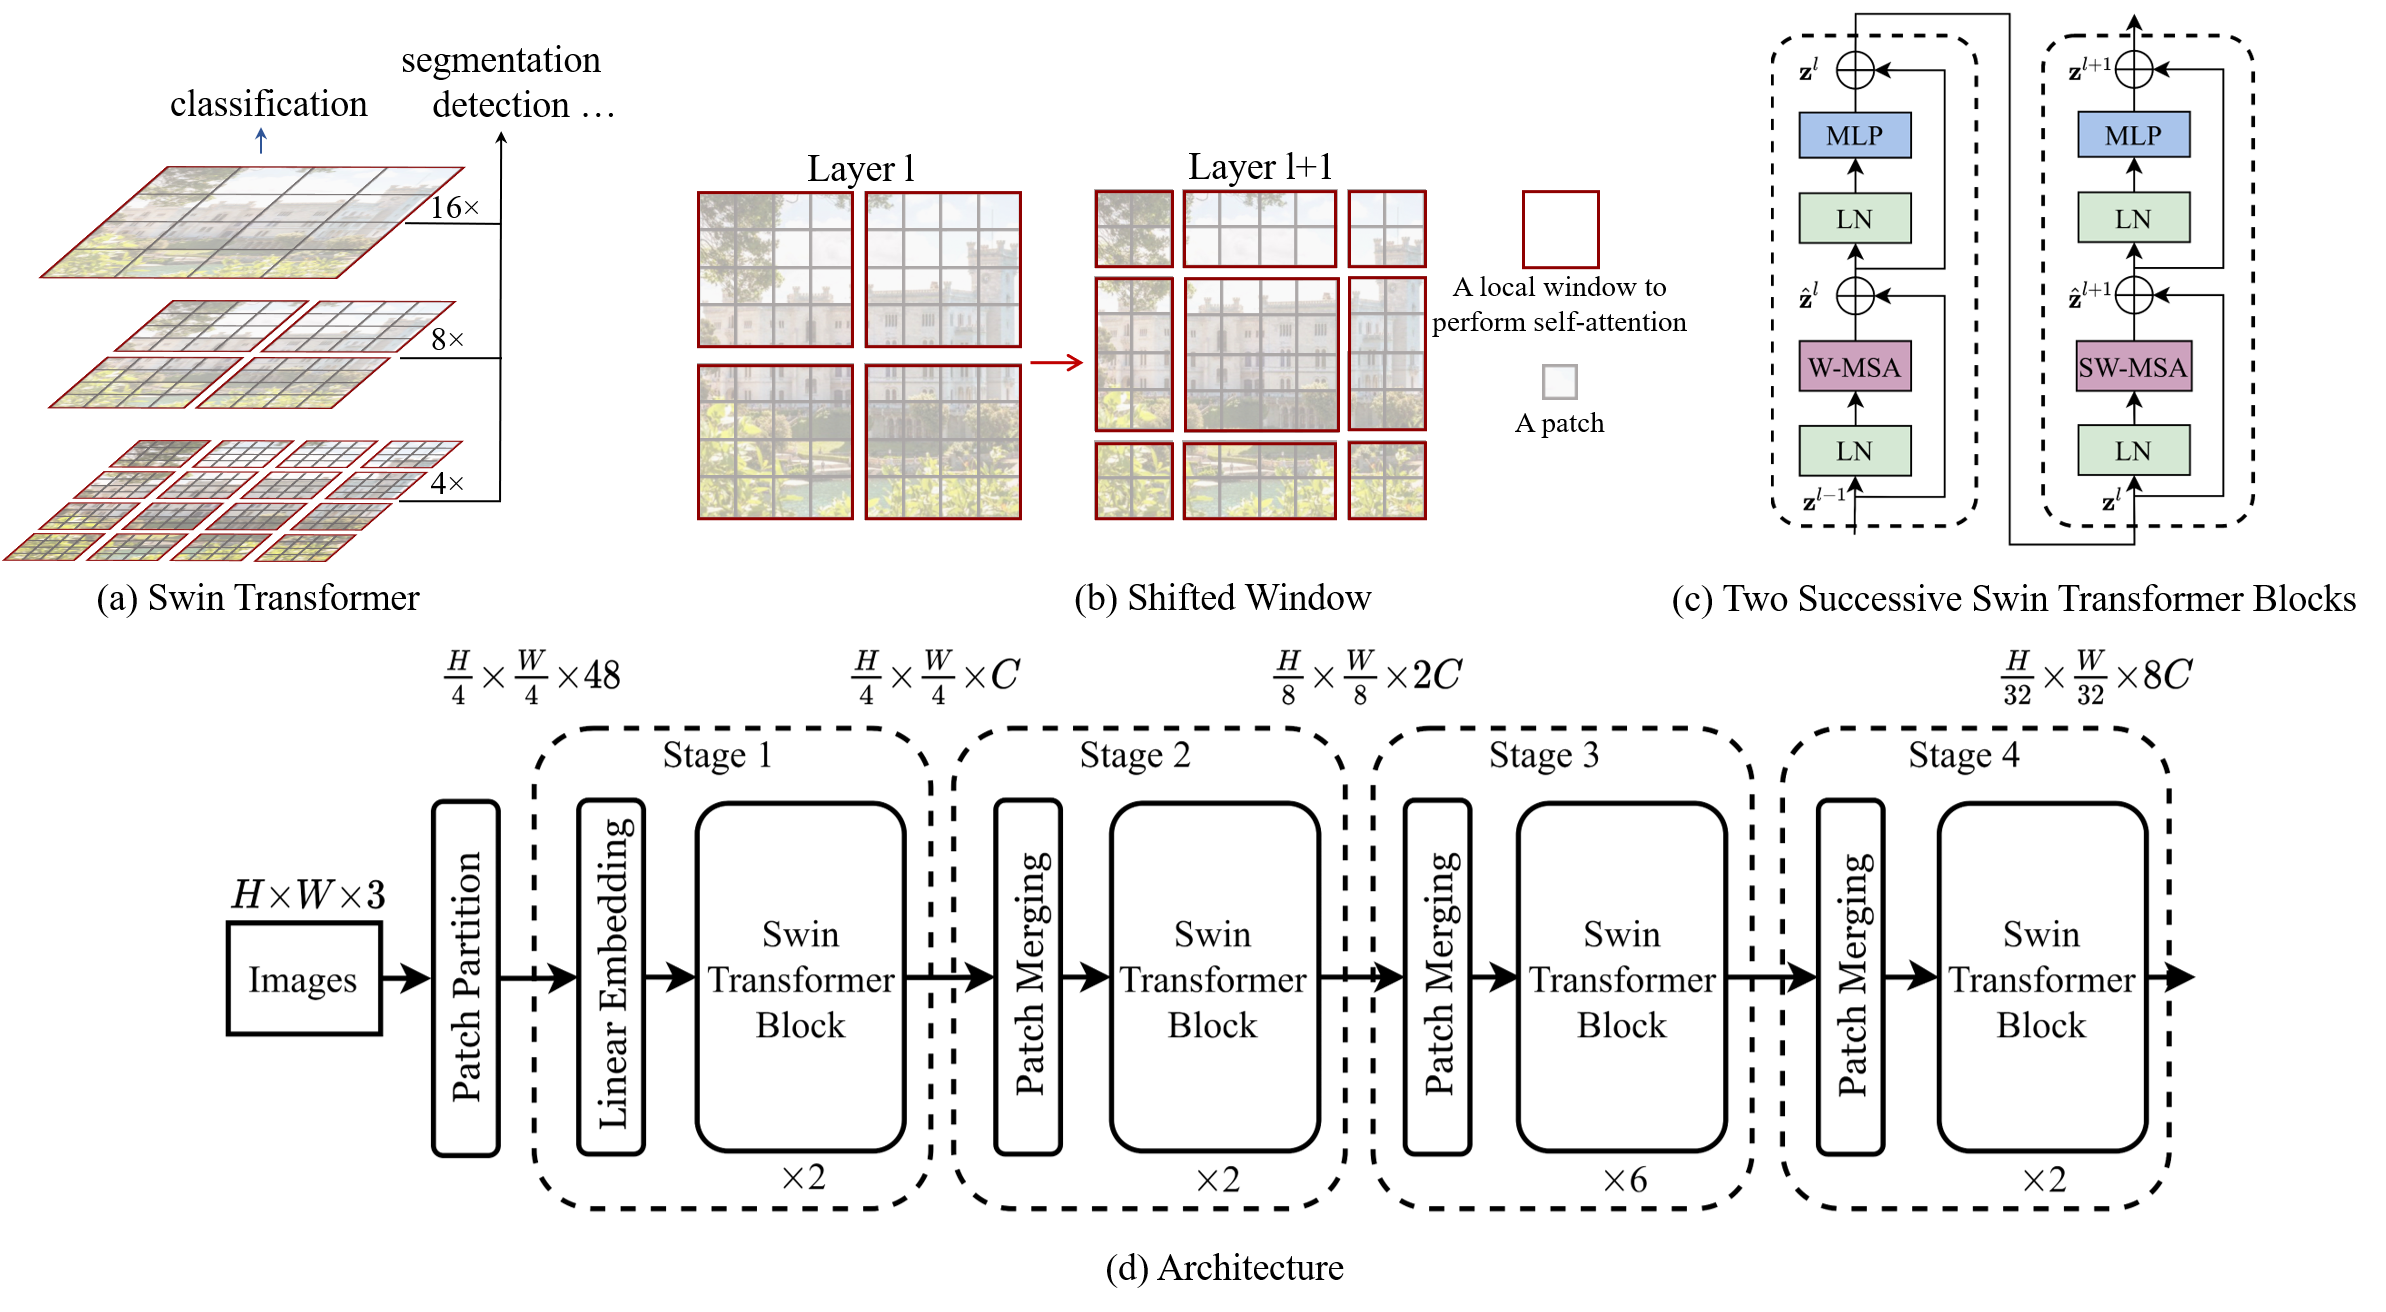
\includegraphics[width=\textwidth]{transformer_images/swin_transformer.png}
		\caption{Swin Transformer}
		\label{fig:Cls Token In Vision Transformer}
	\end{minipage}
	\hfill
	
\end{figure}


در Swin Transformer به جای آنکه مدل به تمام پَچ‌ها در سطح ویژگی نگاه کند، تصویر را به “پنجره‌های محلی” (Local Windows) تقسیم می‌کند و توجه خود را محدود به همان ناحیه می‌کند. 

 سپس با تکنیک جابه‌جایی (Shift) این پنجره‌ها در لایه‌های بعدی، توان مدل برای ترکیب اطلاعات از نواحی مختلف تصویر (و در نهایت دیدن کل تصویر) افزایش پیدا می‌کند. این رویکرد، ایدهٔ کلیدی بود که باعث شد مدل هم محاسبات سبک‌تر شود و هم همچنان ارتباط‌های جهانی (Global) را در طول لایه‌ها به‌دست آورد.


یکی دیگر از ایده‌های مهم در Swin، کوچک کردن تدریجی نقشهٔ ویژگی (Feature Map) در طول معماری است، شبیه به کاری که در ResNet یا سایر CNNها انجام می‌شود. این موضوع ضمن کاهش هزینهٔ محاسباتی، باعث می‌شود مدل بتواند با سطوح مختلفی از ویژگی‌ها کار کند و در نهایت خروجی نهایی باکیفیت‌تری ارائه دهد.

   
   
\subsection{ قطعه‌بندی پچ (Patch Partition):}

فرض میکنیم  تصویر ورودی \(\displaystyle I\) دارای ابعاد \(\displaystyle (H \times W \times 3)\) باشد. گام نخست، تقسیم تصویر به پچ‌های کوچک \(\displaystyle (P \times P)\) است. اگر \(P\) اندازهٔ پچ (Patch size) باشد، آنگاه تعداد پچ‌ها در بعد افقی و عمودی، به‌ترتیب \(\displaystyle \frac{H}{P}\) و \(\displaystyle \frac{W}{P}\) خواهد بود. هر پچ را می‌توان به‌صورت یک بردار درآورد:


\[
X_{\text{patch}} \in \mathbb{R}^{(P^2 \cdot 3)}.
\]


سپس کل تصویر به \(\displaystyle \frac{H}{P} \times \frac{W}{P}\) پچ تبدیل خواهد شد و در نتیجه، ماتریس \(\displaystyle X\) از کنار هم قرار گرفتن این پچ‌ها به صورت زیر به‌دست می‌آید:

\[
X \in \mathbb{R}^{\left(\frac{H}{P} \cdot \frac{W}{P}\right) \times \left(P^2 \cdot 3\right)}.
\]


\subsection{Linear Embedding:}

در ادامه برای این‌که بتوانیم هر پچ را در یک فضای برداری با بعد \(\displaystyle C\) (ابعاد مدل) نمایش دهیم، 
یک لایهٔ خطی (Fully Connected Layer) روی هر پچ اعمال می‌شود:


\[
Z = X \cdot W_{\text{embed}} + b_{\text{embed}}, 
\quad
Z \in \mathbb{R}^{\bigl(\tfrac{H}{P} \cdot \tfrac{W}{P}\bigr) \times C}.
\]
در عمل، این عملیات معادل یک تبدیل خطی ساده است:
\[
W_{\text{embed}} \in \mathbb{R}^{\bigl(P^2 \cdot 3\bigr) \times C},
\quad
b_{\text{embed}} \in \mathbb{R}^{C}.
\]
    
پس از این مرحله، ما در هر موقعیت \((h, w)\) (از شبکهٔ پچ‌ها) یک بردار 
\(\displaystyle z_{h,w} \in \mathbb{R}^{C}\) داریم. این ماتریس \(\displaystyle Z\) 
ورودیِ اولین مرحله (Stage) از Swin Transformer است.



هر بلوک swin transformer  از دو بخش اصلی تشکیل شده است.

\begin{itemize}
	\item پنجره‌بندی تصویر (\textbf{Window Partition}) 
	یا پنجره‌بندی جابه‌جاشده (\textbf{Shifted Window Partition})
	
	\item اعمال \(\mathrm{WMSA}\) (\textbf{Window Multi-Head Self Attention})
	
	\item لایهٔ \textbf{Skip Connection} و \textbf{Layer Norm}
	
	\item مسیر \textbf{MLP}:
	\begin{itemize}
		\item یک لایهٔ MLP شامل دو لایهٔ \textbf{Fully-Connected} 
		و تابع فعال‌ساز \textbf{GeLU} (یا تابع مشابه)
		\item لایهٔ \textbf{Skip Connection} و \textbf{Layer Norm}
	\end{itemize}
\end{itemize}



\subsection{Window Multi-Head Self-Attention:}


\subsubsection{ تعریف پنجره‌های محلی:}

در Swin Transformer، به‌جای آن‌که تمام پیکسل‌های یک نقشهٔ ویژگی بزرگ را یک‌جا 
در محاسبهٔ Attention درگیر کنیم، نقشهٔ ویژگی را به قطعه‌های کوچکی به‌اندازهٔ 
\(\displaystyle (M \times M)\) تقسیم می‌کنیم. این قطعه‌های کوچک را 
«پنجره‌های محلی» می‌نامیم.

اگر اندازهٔ نقشهٔ ویژگی در یک لایه 
\(\displaystyle (H' \times W')\) باشد، 
با تقسیم آن به پنجره‌های 
\(\displaystyle (M \times M)\)، 
در راستای طول تقریباً 
\(\displaystyle \tfrac{H'}{M}\) پنجره خواهیم داشت 
و در راستای عرض هم 
\(\displaystyle \tfrac{W'}{M}\) پنجره.
(برای راحتی، فرض می‌کنیم 
\(\displaystyle H'\) و \(\displaystyle W'\) 
دقیقاً مضربی از \(\displaystyle M\) باشند 
تا تقسیم بدون باقی‌مانده انجام شود.)

هر کدام از این پنجره‌های 
\(\displaystyle (M \times M)\) 
دارای 
\(\displaystyle M^2\) پیکسل (یا موقعیت مکانی) است، 
و در هر پیکسل هم یک بردار ویژگی با بعد \(\displaystyle C\) قرار دارد.

به بیان ساده‌تر:
\begin{itemize}
	\item نقشهٔ ویژگی مثل یک صفحهٔ بزرگ است.
	\item آن را مانند شطرنج به مربع‌های کوچکی \(\displaystyle (M \times M)\) بخش می‌کنیم.
	\item در هر مربع (پنجره)، فقط به همان مربع نگاه می‌کنیم و محاسبات Attention را انجام می‌دهیم.
	\item این کار باعث می‌شود تعداد پیکسل‌هایی که درگیر محاسبهٔ Attention هستند، 
	به‌مراتب کمتر شود و هزینهٔ محاسباتی کاهش یابد.
\end{itemize}


\subsection{Attention:}

برای هر بلوک، ابتدا بردارهای \textbf{Query}، \textbf{Key} و \textbf{Value} ساخته می‌شوند. 
اگر \(\displaystyle z_i \in \mathbb{R}^C\) بردار ورودی مربوط به موقعیت \(i\) باشد، آنگاه:

\[
q_i = z_i W_Q, 
\quad
k_i = z_i W_K,
\quad
v_i = z_i W_V,
\]
که 
\[
W_Q, W_K, W_V \;\;\in \;\;\mathbb{R}^{C \times d}.
\]
پارامتر \(\displaystyle d\) معمولاً \(\displaystyle \tfrac{C}{h}\) در نظر گرفته می‌شود 
و \(\displaystyle h\) تعداد سربندی (\textit{Head})ها است. 
در \textbf{Multi-Head Attention}، خروجی نهایی با ترکیب \(\displaystyle h\) سر توجه محاسبه می‌شود.

در یک سر توجه، توجه به‌صورت زیر تعریف می‌شود:

\[
\mathrm{Attention}(Q, K, V)
=
\mathrm{Softmax}\Bigl(\frac{QK^\top}{\sqrt{d}}\Bigr)\,V,
\]

که در آن:

\begin{itemize}
	\item \(\displaystyle Q, K, V\) به‌ترتیب ماتریس‌هایی هستند که از کنار هم قرار دادن 
	\(\displaystyle q_i, k_i, v_i\) (برای تمام پیکسل‌های آن پنجره) ساخته می‌شوند.
	\item \(\displaystyle \sqrt{d}\) عامل مقیاس‌کننده برای جلوگیری از بزرگ شدن بیش‌ازحد ضرب داخلی است.
\end{itemize}

در \textbf{Swin Transformer}، این محاسبات به‌صورت پنجره‌ای انجام می‌شوند؛ یعنی 
برای هر پنجره، تنها پیکسل‌های داخل همان پنجره در ماتریس‌های 
\(\displaystyle Q\) و \(\displaystyle K\) و \(\displaystyle V\) لحاظ می‌شوند. 
به این ترتیب، زمان محاسبه و مصرف حافظه به‌شدت کاهش می‌یابد 
(در مقایسه با \textbf{ViT} که همه‌چیز را با هم مقایسه می‌کند).

تعداد سربندی \(\displaystyle h\) معمولاً طوری انتخاب می‌شود که 
\(\displaystyle C = h \times d.\) 
خروجی هر سر پس از محاسبهٔ Attention به‌صورت زیر با هم ادغام می‌شوند:

\[
\mathrm{MultiHead}(Q,K,V) 
= 
\bigl[\text{head}_1,\ \text{head}_2,\ \dots,\ \text{head}_h\bigr]\,
W_O,
\]
که 
\[
\text{head}_j = \mathrm{Attention}\bigl(Q_j,\ K_j,\ V_j\bigr),
\quad 
W_O \in \mathbb{R}^{C \times C}
\]
ماتریس ترکیب نهایی است.
\subsection{shifted Windows:}


در \textbf{Swin Transformer}، ایدهٔ «پنجره‌های جابه‌جاشده» (\textit{Shifted Windows}) 
به این منظور ارائه شده است تا مدل، ارتباط پیکسل‌های واقع در پنجره‌های مجاور را هم یاد بگیرد. 
اگر فقط از پنجره‌های ثابت (بدون جابه‌جایی) استفاده کنیم، هر بلوک از تصویر تنها با پیکسل‌های همان 
پنجره در ارتباط خواهد بود و ممکن است اطلاعات نواحی مرزی با نواحی مجاور به‌خوبی تبادل نشود. 

روش \textbf{Swin} برای رفع این محدودیت از یک تکنیک ساده اما مؤثر استفاده می‌کند:
\begin{itemize}
	\item در یک لایه، محاسبات Attention در پنجره‌های محلی ثابت انجام می‌شود.
	\item در لایهٔ بعدی، پنجره‌ها به اندازه‌ای مشخص جابه‌جا می‌شوند (به‌صورت شیفت افقی و عمودی) 
	تا نواحی مرزی نیز در محاسبات گنجانده شوند.
	\item این فرآیند باعث می‌شود که پیکسل‌ها در پنجره‌های مختلف (و در مرزهای مختلف) 
	در محاسبات دخیل شوند و تبادل اطلاعات بهتری میان نواحی تصویر رخ دهد.
\end{itemize}


\subsubsection{بلوک اول (W-MSA):}

در این بلوک، نقشهٔ ویژگی به پنجره‌های \(\displaystyle (M \times M)\) تقسیم می‌شود. 
هیچ جابه‌جایی در این تقسیم‌بندی وجود ندارد؛ یعنی اگر نقشهٔ ویژگی را یک مستطیل بزرگ در نظر بگیریم، 
آن را شبیه کاشی‌کاری یا شطرنج‌بندی به بلوک‌های مربعی \(\displaystyle (M \times M)\) برش می‌زنیم. 
در این حالت، پیکسل‌های هر پنجره فقط با همدیگر (درون همان پنجره) ارتباط برقرار می‌کنند 



\subsubsection{بلوک دوم (SW-MSA):}


 مطابق تصویر ... بعد از اینکه بلوک اول کارش تمام شد، در بلوک دوم، قبل از تقسیم‌بندی به پنجره‌های 
\(\displaystyle (M \times M)\)، نقشهٔ ویژگی را جابه‌جا (\textit{Shift}) می‌کنیم. 
در مقالهٔ اصلی، این مقدار جابه‌جایی معمولاً نیمِ اندازهٔ پنجره 
\(\displaystyle \frac{M}{2}\) 


\begin{figure}[h]
	\centering
	\begin{minipage}[b]{1\textwidth}
		\centering
		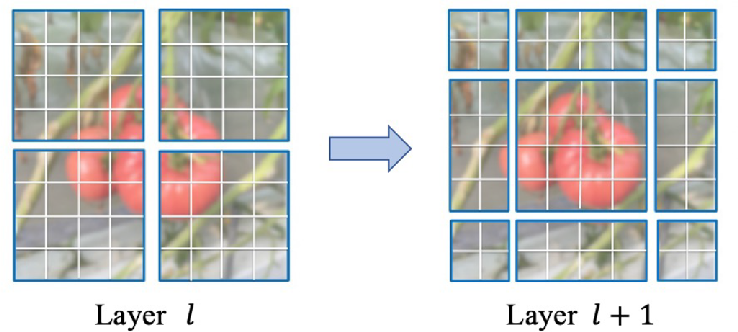
\includegraphics[width=\textwidth]{transformer_images/local_window_with_shifted_local_window.png}
		\caption{Widow vs Shifted Window}
		\label{fig:window vs Shifted Window in Swin Transformer}
	\end{minipage}
	\hfill
	
\end{figure}
در راستای افقی و عمودی است. به این ترتیب:

\begin{itemize}
	\item پیکسل‌هایی که پیش از این در دو پنجرهٔ جداگانه قرار داشتند، ممکن است حالا به دلیل جابه‌جایی وارد یک پنجرهٔ مشترک شوند.
	\item مدل حالا می‌تواند بین این پیکسل‌های «مرزی» نیز Attention برقرار کند و اطلاعات را بهتر مبادله کند.
\end{itemize}

با این جابه‌جایی، بخشی از پیکسل‌ها در نقشهٔ ویژگی از یک طرف «خارج» می‌شوند. برای اینکه این پیکسل‌ها را از دست ندهیم، از ترفندی به نام Cyclic Shift استفاده می‌شود. در Cyclic Shift، پیکسل‌هایی که از سمت راست بیرون می‌روند دوباره از سمت چپ وارد می‌شوند و بالعکس؛ درست شبیه وقتی که یک تصویر را به‌صورت حلقه‌ای اسکرول می‌کنیم (Wrap around). 
مثالی از cycle shift  در تصویر زیر 



\begin{figure}[h]
	\centering
	\begin{minipage}[b]{1\textwidth}
		\centering
		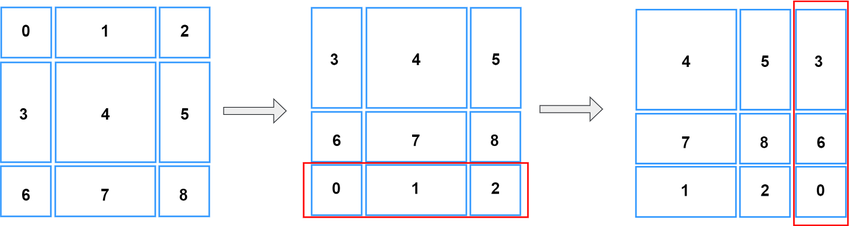
\includegraphics[width=\textwidth]{transformer_images/cycle_shift.png}
		\caption{cycle Shift}
		\label{fig:Cycle Shift in Swin Tranformer}
	\end{minipage}
	\hfill
	
\end{figure}


در بلوک اول (بدون جابه‌جایی)، پنجره‌ها ثابت‌اند و پیکسل‌های مرزی در هر پنجره ممکن است فرصت کافی برای تبادل اطلاعات با پیکسل‌های مرزیِ پنجرهٔ کناری را نداشته باشند.

در بلوک دوم (جابه‌جاشده)، مرزهای پنجره‌ها تغییر می‌کند و برخی پیکسل‌هایی که قبلاً در پنجره‌های جدا بودند، اکنون در یک پنجرهٔ مشترک‌اند؛ در نتیجه مدل می‌تواند رابطه و همبستگی بین آن‌ها را هم یاد بگیرد.

این جابه‌جایی و قرارگیری مجدد پیکسل‌ها کنار هم در نهایت کمک می‌کند تا مدل بتواند اطلاعات کل تصویر را با هزینهٔ محاسباتی کمتر (نسبت به توجهِ سراسریِ کامل) در اختیار داشته باشد.



اگر بخواهم با مثال توضیح دهم فرض کنید در یک تابلوی شطرنجی، خانه‌های کناری همدیگر را «نمی‌بینند» چون در دو بلوک مختلف هستند. 
اما اگر کمی تابلوی شطرنجی را به سمت بالا-چپ یا پایین-راست جابه‌جا کنیم، 
حالا بخشی از آن خانه‌ها وارد یک بلوک واحد می‌شوند و اطلاعاتشان با هم ترکیب می‌شود. 
سپس به‌طور دوره‌ای (\textit{Cyclic})، گوشه‌های اضافی را به آن سمت دیگر تابلوی شطرنجی می‌آوریم 
تا هیچ چیز از دست نرود. 

به این شکل، سِری اول و دوم بلوک‌های \textbf{Swin Transformer} (\textbf{W-MSA} و \textbf{SW-MSA}) 
تکمیل‌کنندهٔ یکدیگر می‌شوند:

\begin{itemize}
	\item \textbf{بلوک اول:} محاسبهٔ Attention در چهارچوب پنجره‌های ثابت.
	\item \textbf{بلوک دوم:} محاسبهٔ Attention در پنجره‌های جابه‌جاشده که منجر به تعامل بیشتر بین مرزهای مختلف می‌شود.
\end{itemize}


\subsection{Mlp:}


پس از انجام \textit{Window (یا Shifted Window) Multi-Head Self-Attention}، 
خروجی به یک مسیر \textbf{MLP} می‌رود. ساختار این MLP به‌صورت زیر است:

\[
X' = \mathrm{GELU}(X W_1 + b_1) W_2 + b_2,
\]

که:
\[
W_1 \in \mathbb{R}^{C \times (rC)}, 
\quad
W_2 \in \mathbb{R}^{(rC) \times C}
\]
هستند و \(\displaystyle r\) معمولاً ضریب افزایش بعد را نشان می‌دهد (مثلاً ۴). 

\textbf{GELU}، \textbf{ReLU} یا سایر توابع فعال‌ساز نیز در اینجا قابل استفاده هستند.

\subsection{patch merging:}

در مدل Swin Transformer، ساختار سلسله‌مراتبی به این معناست که ما در چند مرحله (Stage) مختلف، نقشهٔ ویژگی (Feature Map) را کوچک‌تر می‌کنیم و در عین حال، عمق (تعداد کانال‌های ویژگی) را افزایش می‌دهیم. هدف از این کار دو چیز است:



\textbf{استخراج ویژگی‌های سطح بالاتر:} 
وقتی نقشهٔ ویژگی کوچک‌تر می‌شود، هر واحد از نقشهٔ ویژگی بیانگر بخش گسترده‌تری از تصویر اصلی است؛ 
پس مدل به‌تدریج جزئیات محلی را با درک کلی‌تری از تصویر جایگزین می‌کند.

\textbf{کاهش هزینهٔ محاسبات:} 
در مراحل بعدی، چون ابعاد فضایی کمتر می‌شود، مدل راحت‌تر می‌تواند با ویژگی‌های جدید کار کند 
(چون حالا مثلاً به‌جای \((H \times W)\) پیکسل، تعداد کمتری پیکسل داریم).

این فرایند کوچک‌سازی در \textbf{Swin Transformer} با نام \textit{Patch Merging} شناخته می‌شود 
که شبیه به \textit{Downsampling} در شبکه‌های کانولوشنی (مثل \textit{Pooling} یا \textit{Stride-Convolution}) عمل می‌کند.


 
ابعادی به شکل \((\tfrac{H}{P}, \tfrac{W}{P})\) با تعداد کانال \(\displaystyle C\) دارد. 
این یعنی پس از برش‌دادن تصویر به پچ‌ها و یک یا چند بلوک پردازشی، اکنون یک نقشهٔ ویژگی داریم که کوچک‌تر از تصویر اصلی است، 
اما هنوز ممکن است خیلی بزرگ باشد.

در مرحلهٔ بعدی (\textit{Stage} بعد)، می‌خواهیم این نقشه را نصف کنیم 
(یعنی طول و عرض را دو برابر کوچک کنیم) و در عوض عمق کانال را دو برابر کنیم 
(تا ظرفیت مدل در استخراج ویژگی‌های پیچیده‌تر بیشتر شود). برای انجام این کار از یک فرایند به نام 
\textbf{Patch Merging} استفاده می‌کنیم:

\subsubsection{1. انتخاب بلوک‌های \((2 \times 2)\)}
ابتدا نقشهٔ ویژگی را به بلوک‌های \((2 \times 2)\) تقسیم می‌کنیم (در بُعد مکانی). 
اگر \(\displaystyle Z_{i,j}\) ویژگیِ مکان \((i, j)\) باشد، 
یک بلوک \((2 \times 2)\) شامل چهار پیکسل است:

\[
Z_{2i, 2j}, \quad Z_{2i, 2j+1}, \quad Z_{2i+1, 2j}, \quad Z_{2i+1, 2j+1}.
\]

\subsubsection{2. ادغام (Concat) ویژگی‌های چهار پیکسل}
برای هر بلوک \((2 \times 2)\)، این چهار پیکسل را به هم می‌چسبانیم (\textit{Concat}) در بُعد کانال. 
اگر هر پیکسل یک بردار از بعد \(\displaystyle C\) باشد، حالا بعدِ حاصل از این چهار پیکسل کنار هم می‌شود \(\displaystyle 4C\). 
نام این بردار ادغام‌شده \(\displaystyle Z'\) است.

\subsubsection{3. لایهٔ خطی برای تغییر بعد}
وقتی چهار بردار \(\displaystyle C\)-بعدی را کنار هم گذاشته‌ایم، یک بردار \(\displaystyle 4C\)-بعدی شکل گرفته است. 
حال با یک لایهٔ خطی (\textit{Fully Connected})، بعدِ \(\displaystyle 4C\) را به بعد جدیدی تبدیل می‌کنیم. 
معمولاً این بعد جدید برابر \(\displaystyle 2C\) در نظر گرفته می‌شود؛ 
یعنی می‌خواهیم دو برابر بزرگ‌تر از قبل باشد اما نه چهار برابر:

\[
Z' \mapsto Z'' = Z' W_{\text{merge}} + b_{\text{merge}},
\]

که باعث می‌شود بُعد ویژگی از \(\displaystyle 4C\) به \(\displaystyle 2C\) کاهش یابد.

\subsubsection{4. کاهش ابعاد مکانی}
در عین حال، وقتی هر چهار پیکسل \((2 \times 2)\) را در یک ادغام می‌کنیم، 
یعنی نقشهٔ ویژگی فضای \((\tfrac{H}{2P} \times \tfrac{W}{2P})\) پیدا می‌کند 
(چون هر بلوک \((2 \times 2)\) تبدیل به یک بردار می‌شود).

به عبارت دیگر، تعداد نقاط مکانی نصف می‌شود (هم در طول و هم در عرض)، 
اما کانال از \(\displaystyle C\) به \(\displaystyle 2C\) افزایش می‌یابد.


\begin{figure}[h]
	\centering
	\begin{minipage}[b]{1\textwidth}
		\centering
		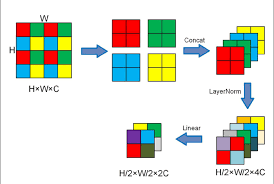
\includegraphics[width=\textwidth]{transformer_images/patch_merging.png}
		\caption{Patch Merging}
		\label{fig:patch merging in Swin Transformer}
	\end{minipage}
	\hfill
	
\end{figure}

در شبکه‌های کانولوشنی، ما مرتباً با لایه‌های \textit{Pooling} یا \textit{Convolution} 
با استراید ۲ روبه‌رو می‌شویم تا ابعاد فضایی را پایین بیاوریم و در عوض تعداد کانال‌ها را بالا ببریم. 
این کار کمک می‌کند اطلاعات سطح بالاتر (مانند ساختار کلی اشیا) راحت‌تر استخراج شود. 
\textbf{Swin Transformer} هم از همین ایدهٔ سلسله‌مراتب الهام گرفته است. 
همچنین اگر ابعاد فضایی را پیوسته پایین نیاوریم، هزینهٔ \textit{Attention} به‌شدت زیاد می‌شود 
(چون در هر لایه باید محاسبهٔ Attention برای همهٔ پیکسل‌ها انجام شود).

در معماری کلی \textbf{Swin Transformer}، در \textit{Stage 1} ویژگی‌های اصلی گرفته می‌شود 
و بعد از گذر از \textbf{W-MSA} و \textbf{SW-MSA}، عملیات \textbf{Patch Merging} انجام می‌شود. 
حالا در \textit{Stage 2} ویژگی‌های کوچک‌تری داریم، اما تعداد کانال‌ها افزایش یافته است. 

مطابق آن‌چه در کانولوشن داریم، با افزایش عمق، تعداد ویژگی‌ها کمتر و تعداد کانال‌ها افزایش پیدا می‌کند.


و در نهایت پس از stage  آخر به یک لایه FC  برای متصل میشود. و نتیجه کلاس ها پس از عبور از Softmax  به ما داده میشود.





